\documentclass[12pt]{article}
\usepackage{graphicx,subfigure}
\usepackage{hyperref,amsmath,fancyhdr}
\usepackage[usenames,dvipsnames]{color}
\usepackage{supertabular}
\usepackage[english]{babel} 
%\usepackage[left=2.0cm, right=2.0cm, top=2.5cm, bottom=2.5cm, headsep=1.2cm]{geometry}
\usepackage{amscd,amssymb,verbatim}
%\usepackage[TS1,OT1,T1]{fontenc}
\usepackage{cite}
\usepackage{eurosym}
\usepackage{array}
\usepackage{hyperref}
\usepackage{fancyvrb}
\usepackage{multirow}
\usepackage[titletoc]{appendix}
\usepackage{ccaption}
\pagestyle{headings}
\usepackage{subfigure} 
\usepackage{color}
 
\textheight 23cm
\textwidth 17.5cm
\topmargin -1.0cm
\hoffset -2.0cm

\newfixedcaption{\figcaption}{figure}

\begin{document}

\begin{titlepage}
\centering
{{\Huge\bf \sffamily MINT}}\\
\vspace{0.35cm}
{{\Huge\bf \sffamily version 1.0}}\\
\vspace{0.5cm}
{{\Huge\bf \sffamily Users' Manual}}\\
\vspace{1cm}
{\large{\bf{\sffamily Anna G\'{o}rska}}}\\
{\large{\bf{\sffamily Maciej Jasi\'{n}ski}}}\\
{\large{\bf{\sffamily Joanna Trylska}}}\\
\vspace{2cm}
\includegraphics[width=0.4\textwidth]{./pictures/MINT.png}\\
\vspace{0.2cm}

\includegraphics[width=0.3\textwidth]{./pictures/logoLMB.png}
\end{titlepage}
\newpage
     {\sffamily{The MINT is a free software; you can redistribute it and/or modify 
     it under the terms of the GNU General Public License version 2,  
     as published by the Free Software Foundation.\\
     \\                                                                       
     This program is distributed in the hope that it will be useful,        
     but WITHOUT ANY WARRANTY; without even the implied warranty of       
     MERCHANTABILITY or FITNESS FOR A PARTICULAR PURPOSE.  See the GNU General Public License for more details.\\                          
     \\                                                                       
     You should have received a copy of the GNU General Public License    
     along with this program; if not, write to the                         
     Free Software Foundation, Inc.,                                      
     59 Temple Place - Suite 330, Boston, MA  02111-1307, USA.\\
     \\
     \vspace*{1cm}
     Copyright (C) 2013: University of Warsaw}}  
\includegraphics[width=0.1\textwidth]{./pictures/logoUW.png}

\newpage
\tableofcontents
\newpage
\newcommand*{\elem}[1]{{\color{Gray}{\tt{<#1>}}}}
\newcommand*{\greyT}[1]{{\color{Gray}{\tt{#1}}}}

\section{Introduction}
MINT stands for Motif Identifier for Nucleic acids Trajectory - this is an automatic tool for reading and analyzing RNA three-dimensional structures and molecular dynamics trajectories (written in CHARMM, Gromacs, NAMD, LAMMPS, or Amber formats). The analysis includes RNA hydrogen network pattern and structural motifs. These properties can be investigated as a function of the conformations provided by the user. In the case of molecular dynamics trajectory MINT gives the flow of various RNA properties in time.\\

\noindent
Please direct your comments and questions about the MINT package to:\\
{\tt{agorska@cent.uw.edu.pl}}\\
Centre of New Technologies,
University of Warsaw\\
\.{Z}wirki i Wigury 93, 02-089 Warsaw, Poland\\
phone:  $+$48 22 5540 843 \\ 
\\
The web interface to analyze RNA structures is available at:\\
\\
{\color{Blue}{\tt{{\color{red}https://bionano.cent.uw.edu.pl/MINT}}}}\\
\\
\noindent
and the source code of the MINT package to analyze multiple snapshots, for example, molecular dynamics trajectories can be found at:\\
\\ 
{\color{Blue}{\tt{https://bionano.cent.uw.edu.pl/Software}}}\\
\\
MINT is distributed under the terms of the GNU Public License. 
A copy of the GPL is provided with the distribution and is also available at {\color{Blue}\tt{http://www.gnu.org}}. \\

\noindent
If you find this software useful please cite: Anna G\'{o}rska, Maciej Jasin\'{n}ski, Joanna Trylska, {\color{red}TITLE, JOURNAL, submitted}

\section{Quick reference}
\subsection{What our software can do?}

\textbf{For a single .pdb file of an RNA molecule MINT computes and outputs:}
\begin{itemize}
\item regions forming helices,
\item regions forming loops, bulges, interior loops, junctions,
\item regions forming pseudo-knots,
\item nucleotides creating triplexes,
\item all Watson-Crick base pairs,
\item all non-Watson-Crick base pairs,
\item the number of Watson-Crick hydrogen bonds per nucleotide,
\item the number of non-Watson Crick hydrogen bonds per nucleotide,
\item the stacking energy -- Van der Waals and electrostatic energies and their sum per nucleotide,
\item visualizations of the computed parameters.
\end{itemize}

\textbf{For a trajectory file it computes and outputs:}
\begin{itemize}
\item residues forming helices, triplexes, pseudo-knots and other motifs, as well as frame numbers and percentage of time when they were present, \item clusters of secondary structure motifs and average motifs along with two-dimensional and three-dimensional contacts,
\item all Watson-Crick and non-Watson-Crick base pairs and frame numbers in which a helix was present as well as percentage of trajectory time the helix occurred,
\item the average number of Watson-Crick and non-Watson Crick hydrogen bonds per nucleotide,
\item the average stacking energy -- Van der Waals and electrostatic energies and their sum per nucleotide,
\item average secondary structure,
\item visualizations of the computed parameters (see section \ref{Visualization})
\end{itemize}

\subsection{What does it need?}
\begin{itemize}
\item Python2.7 and described below packages.
\item an RNA structure file in a full-atom (including hydrogens) representation and in the .pdb format.
\item a trajectory file (e.g. in the .dcd format) in case you want to use the \texttt{Traj} mode.
\end{itemize}

\subsection{Example}
On the website we provide an example.tar package containing \textbf{inputs}:
\begin{itemize}
\item \texttt{example.pdb}  -- a pdb file containing the atomic structure of the RNA molecule. One will benefit from the program mostly while analyzing the RNA structures with a complex secondary an tertiary structures.
\item \texttt{example.dcd}  -- a trajectory file containing ten frames from molecular dynamics simulations performed with NAMD \cite{Phillips2005} and using the CHARMM forcefield.
\end{itemize}

and \textbf{outputs}:
\begin{itemize}
\item Structure description (see section \ref{OutputFiles} for details):
\begin{itemize}
\item example\_description			
\item example\_RNA\_ANALIZER.xls	
\item example\_nucleotides\_eval.csv
\item example\_pairs\_in\_time.csv
\item example\_per\_nucleotide.csv
\item example\_average\_motifs.csv		
\item example\_helices\_in\_time.csv		
\item example\_motifs\_clusters.csv
\end{itemize}
\item Visualization  (see section \ref{Visualization} for details):
\begin{itemize}
\item exampleRNAStructML.xml		
\item example\_varna.html
\item example\_2D.pdb				
\item example\_3D.pdb				
\item example\_VDW.pdb				
\item example\_stacking\_sum.pdb
\item example\_coulomb.pdb			
\item vmd\_run.tcl
\end{itemize}
\end{itemize}

All the examples provided in this manual are based on the above example.

\subsection{Running}
After downloading and unpacking the package \texttt{MINT.tar}, you can go straight to the \texttt{MINT} directory and type
\begin{verbatim}
python MINT.py
\end{verbatim}

and the program should perform a single frame analysis of the \texttt{example.pdb}. If any errors appear check whether you are using python2.7 and have all the required packages installed (the packages are listed in the section \ref{external}).

If you would like to perform single frame analysis of your input pdb with hydrogens  

If you want to perform the trajectory analysis of the \texttt{example.dcd} file, type: 
\begin{verbatim}
python MINT.py Single/Traj=Single
\end{verbatim}

Running program with the \texttt{help} option will print all the parameter names and their default values:
\begin{verbatim}
python MINT.py help
\end{verbatim}

To set your own parameters simply type the name of the parameter "=" value list separated with spaces:
\begin{verbatim}
python MINT.py Single/Traj=Traj vmd=0 h\_bond\_angle=130 cutoff=30 threads=1
\end{verbatim}

Another way is to directly edit the  \texttt{parms} dictionary in the end of the \texttt{pairs.py} file in the main function. You can use any text editor but watch out for quotation marks, indents and commas. 


\section{External modules and installation} \label{external}
The script uses several external python packages:
\begin{itemize}
\item python 2.7 -- Python programming language (\url{http://python.org})
\item numpy --  the package containing base tools to manipulate multi-dimensional arrays, the installation is described on the SciPy home website: \url{http://www.scipy.org/Download}
\item BioPython -- the main package that enables loading and managing the PDB structure, the installation is described on the BioPython home website: \url{http://biopython.org/wiki/Main_Page}
\item MDAnalysis \cite{Denning2012} -- used only for reading the trajectory, so as long as a single .pdb file is  analyzed, the \texttt{import MDAnalysis} line can be removed. The instruction how to install this Python package can be found here \url{http://code.google.com/p/mdanalysis/wiki/Install} - MDAnalysis home website. 
\item xlwt -- the package for writing .xls files. It is used by \texttt{csvToxls.py} script to write all output .csv files into the .xls files (can be installed from pypi website \url{https://pypi.python.org/pypi/xlwt}).
\item pympler -- the package enabling measuring the memory use of the objects in python script - can be downloaded from its website \url{http://pythonhosted.org/Pympler/}. 
\end{itemize}

all of them can be installed through \texttt{easy\_install} command available in \texttt{setup\_tools} package (\url{http://pythonhosted.org/distribute/easy_install.html#installing-easy-install}. 

\paragraph{multipy}
If you encounter any kind of problems with installing python2.7 or required packages, you can use a Multipy package. This package allows to set up a local virtual python environment and run the script. The Multipy can be downloaded from the website \url{http://code.google.com/p/multipy/}.  To install python 2.7 type 
\begin{verbatim}
multipy install 2.7
\end{verbatim}
then you can access the python 2.7 multipy environment  by using:
\begin{verbatim}
 bash
 . $(multipy activate 2.7)
\end{verbatim}
and now it is easy to install the needed packages: 
\begin{verbatim}
 easy_install numpy  
 easy_install Biopython
 easy_install MDAnalysis
 easy_install xlwt
 easy_install pympler
\end{verbatim}

\section{Definitions}
Here we outline a few concepts/definitions that we use for the purpose of the manual and running software. The meaning of some has been be narrowed and of others extended in comparison to their biological meaning: 
\begin{itemize} 
\item Canonical pair -- all Watson-Crick pairs, including AG, AC and others.
\item Non-canonical pair -- all non-Watson-Crick pairs.
\item RNA secondary structure -- created by canonical pairs excluding pseudo-knots.
\item RNA tertiary structure -- created only by non-canonical pairs.
\item Motif -- a loop, bulge or junction but not a helix. 
\end{itemize}

\section{Workflow}
Figure \ref{ProgramScheme} shows the structure of the program. First, the program reads in the RNA conformation and finds all hydrogen bonds between nucleotides. They allow determining secondary and tertiary structures and subsequent classification of the RNA secondary structural motifs. The main outcome is a set of statistical descriptors of the given RNA structure. In this document we  describe the algorithm, inputs and outputs of the program. 

\begin{figure}[h!]
\centering
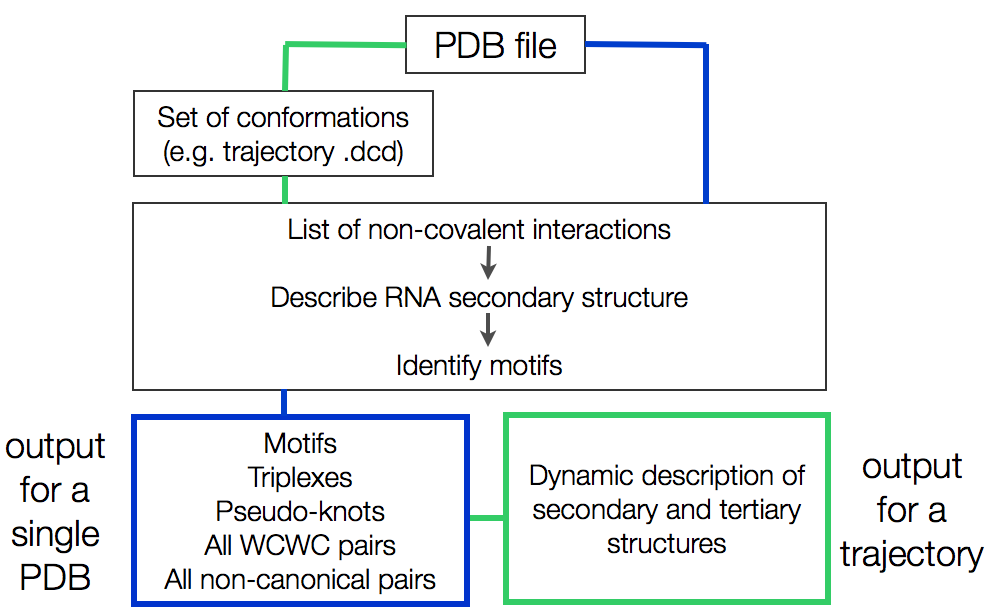
\includegraphics[scale=0.4]{./pictures/workflow.png}
\caption{Main function implements the analysis of a single frame. In the case of a trajectory, the function reads-in the list of nucleotides from a given PDB and then refreshes the atom coordinates while reading the next frame. Additionally, the script splits the trajectory between CPUs and runs separate processes, what  accelerates the calculations.}
\label{ProgramScheme}
\end{figure}

\subsection{Loading the RNA structures}
The script is entirely written in Python programming language (\url{http://python.org}). Its modular structure enables applying it in various programing contexts. Reading the PDB file is implemented  in  BioPython (\url{http://biopython.org/wiki/Main_Page}) package, providing a complete objective structure for dealing with PDBs. The basic object is an atom that despite the name and number is described with coordinates. A molecule consists of the residues that have such attributes as the name, number and list of atoms. This allows fast and easy access to the nucleotides, atoms and their coordinates.

\subsection{Hydrogen bonding}
A hydrogen bond is a basic interaction responsible for creating the RNA secondary and tertiary structures. A typical definition of a hydrogen bond pertains to a non-covalent interaction when a hydrogen atom is placed close to its acceptor.

Both the distance and the angle depend on the characteristics of the donor and acceptor (Figure \ref{hbond}). Theory states that all hydrogen bonds are almost linear (around $175^\circ$) \cite{Guerra2000}. For biological molecules the hydrogen bond distance should be typically between 2,80 and 3,06 \AA\ between a donor and acceptor, which gives 1,60 and 1,80 \AA\ between an acceptor and hydrogen.

The user defines both parameters: the minimal angle and maximal distance of a hydrogen bond. The default value of the h\_bond distance is 2.8 \AA\ and the minimal angle value is $140^\circ$ (see Figure \ref{hbond}).


\begin{figure}[h!]
\centering
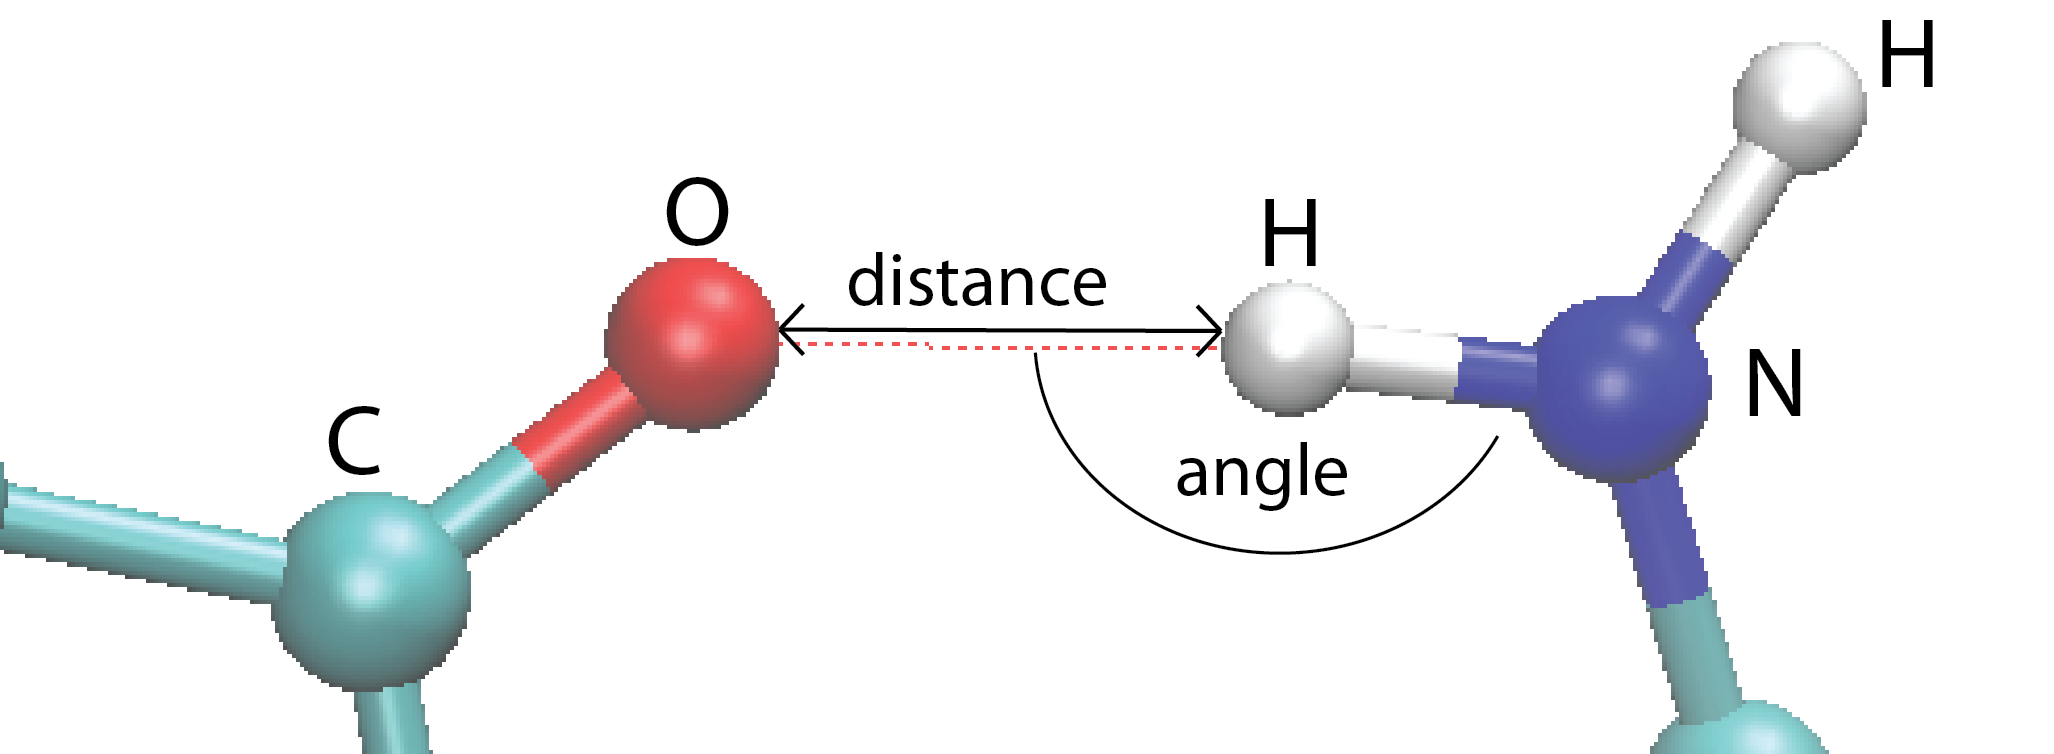
\includegraphics[width = 10cm]{./pictures/hydrogen_bond.png}
\caption{The scheme of the hydrogen bond with the nitrogen atom as a donor and the oxygen atom as an acceptor.}
\label{hbond}
\end{figure}

\subsection{Donors and acceptors}
To analyze the RNA structures we have defined a list of possible acceptors and donors for all four nucleotides (A, U, G, C). Following the classification by Leontis and Westhof \cite{Leontis2002} the acceptors and donors are assigned to the edges of the nucleotide, as shown in  Figure \ref{Edges}. The program determines the interacting edges of every pair of nucleotides. Several atoms are situated in the corners of the nucleotides and participate in more than one edge. In that case, the program first classifies all the remaining bonds and chooses the prevailing edge. If there is only one hydrogen bond, both edge names are returned. 

\begin{figure}[h!]
\centering
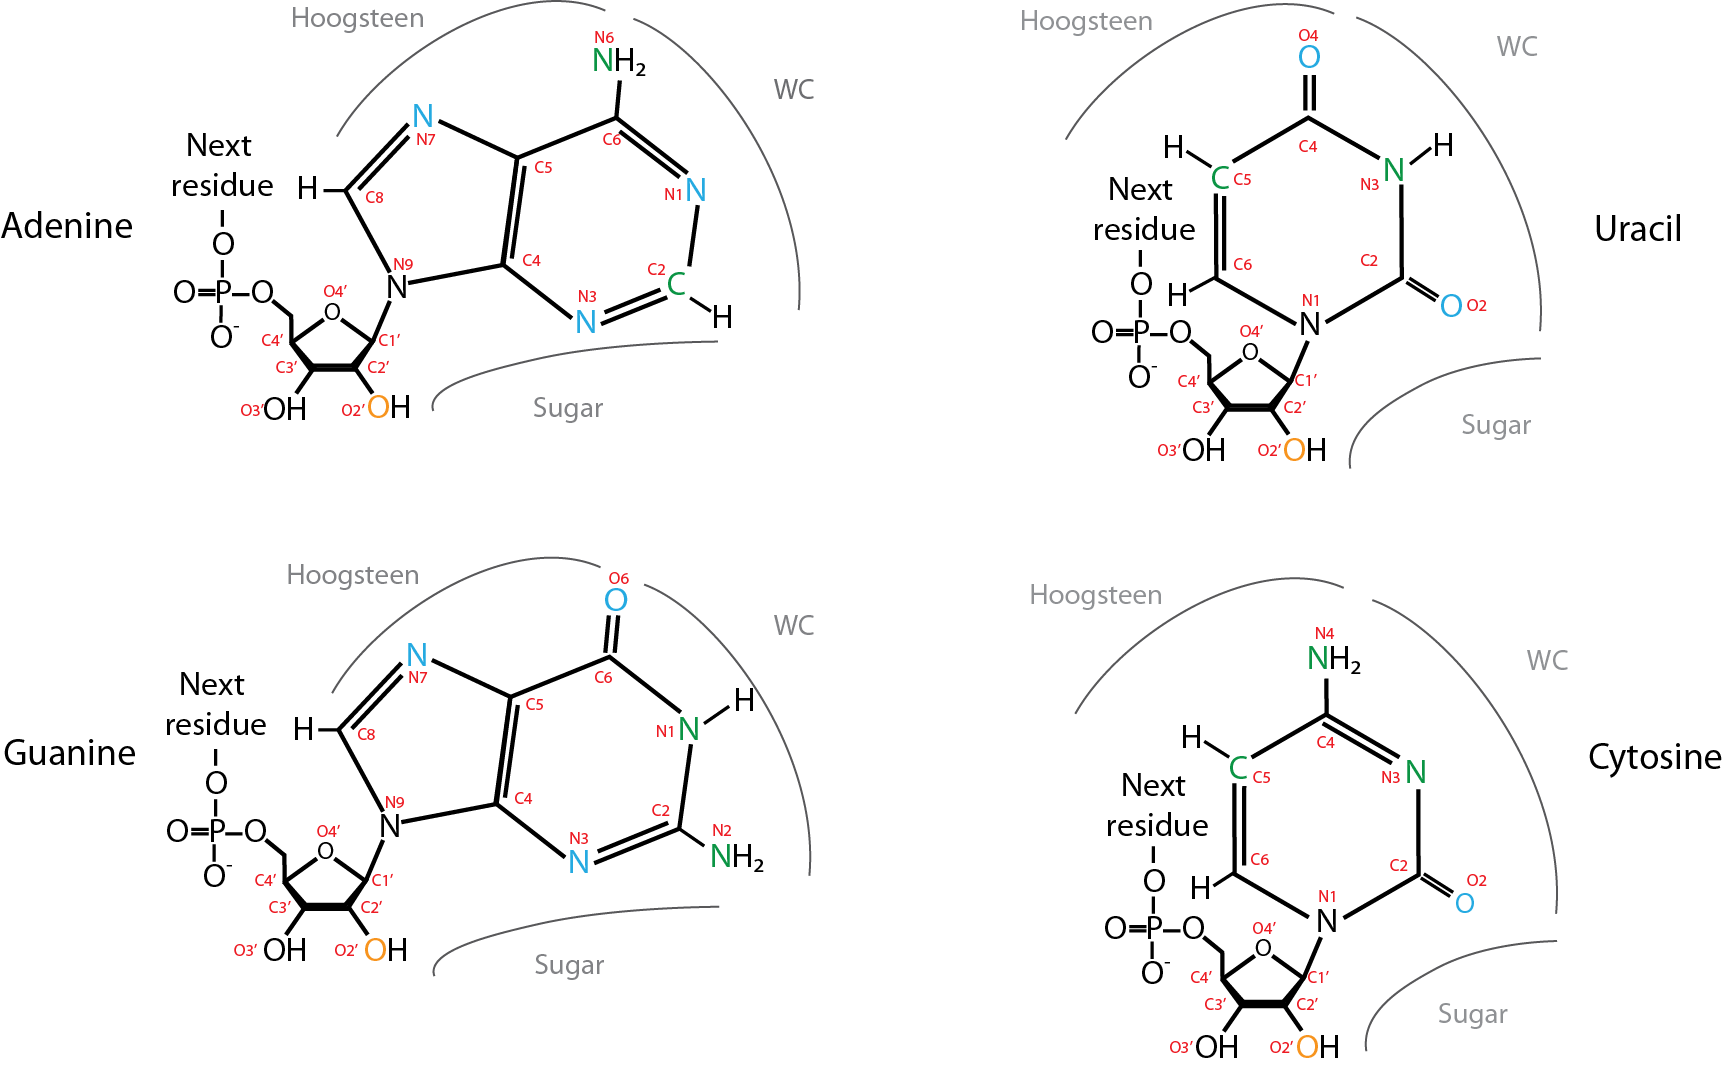
\includegraphics[width = 14cm]{./pictures/donors_acceptors_nucleotides.png}
\caption{Nucleotides with selected edges, donors (green) and acceptors (blue). WC corresponds to Watson-Crick edge.  \cite{Lescoute2006}.}
\label{Edges}
\end{figure}

% Pairs
After determining the donors and acceptors of a molecule, as well as the hydrogen bond pattern, the program can now search for nucleotide pairs. The program has to check all the donors against all acceptors of all possible pairs of nucleotides in the RNA molecule. In order to decrease the computational time, we assumed that the partner for a given nucleotide can be found only among its closest neighbors - nucleotides placed in the space within a given \texttt{cutoff}. The exact distance is defined by the user (\texttt{cutoff}). Knowing the atoms participating in hydrogen bonds, the program can determine the interacting edges.

\paragraph{Modified nucleotides}
RNA structures sometimes include modified nucleotides such as 2N-methylguanosine-5'-monophosphate, 5,6-dihydrouridine-5'-monophosphate or N2-dimethylguanosine-5'-monophosphate that can be found, for example, in tRNA molecules. Several of these are presented in Figure \ref{ModifiedNucleotides}. If you find modified nucleotides in the studied RNA system you should edit the \texttt{nucleotides.csv} file and add  a new row with the name of your residue and appropriate names of atoms in the donors and acceptors columns. Than you should also modify the \texttt{charges\_and\_VDW} file for stacking computation. We could not have done it for you due to the not unified naming of the modified nucleotides and atoms they consist of. 

\begin{figure}[h!]
\centering
\begin{center}
\subfigure[2MG]{
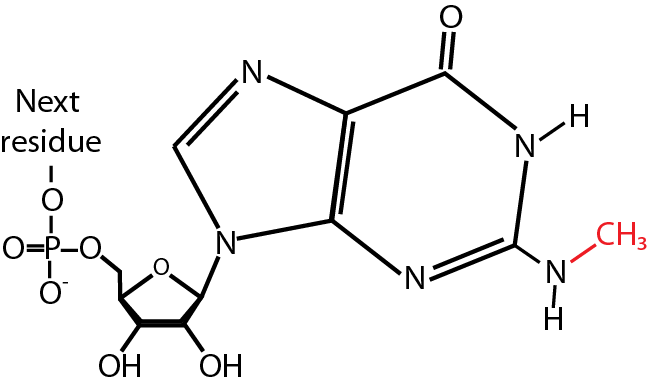
\includegraphics[scale=0.8]{./pictures/modified_1.png}}
\subfigure[OMC]{
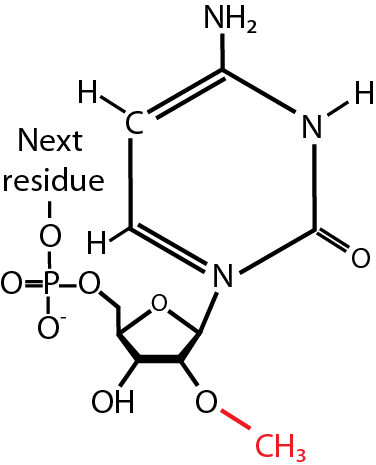
\includegraphics[scale=0.8]{./pictures/modified_2.png}}
\subfigure[YYG]{
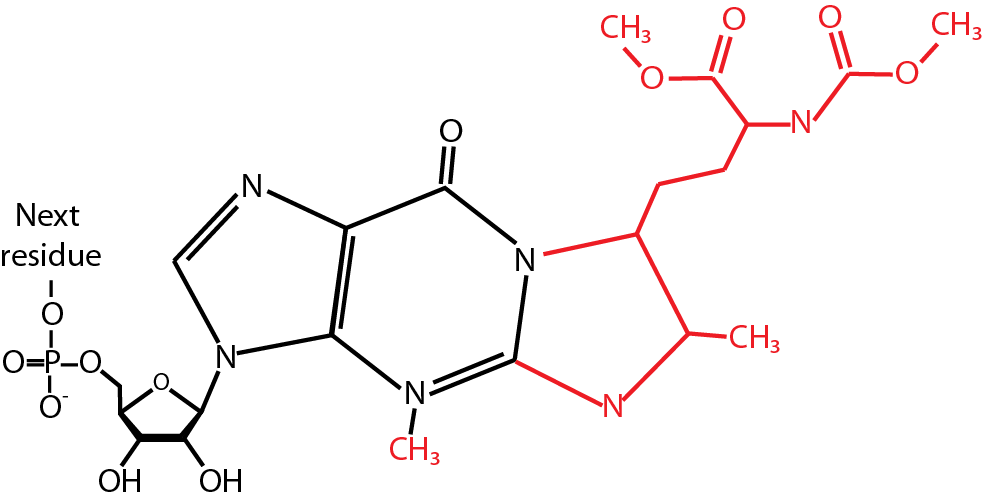
\includegraphics[scale=0.8]{./pictures/modified_3.png}}
\end{center}
\caption{Three out of ten modified nucleotides present in tRNA structure (PDB: 1ttt) along with their PDB ID. Red color indicates atoms that are not present in normal nucleotides. }
\label{ModifiedNucleotides}
\end{figure}

\newpage
%Configuration
\paragraph{Geometric isomerism}
After detecting the hydrogen bonds, and defining the interacting sites, the geometric isomerism is computed. The program measures the torsion angle formed by four atoms, and depending on its value the geometric isomerism is denoted. There are two possible isomerisms: cis and trans, both shown in Figure \ref{Conf}.

\begin{figure}[h!]
\begin{center}
\subfigure[Cis]{
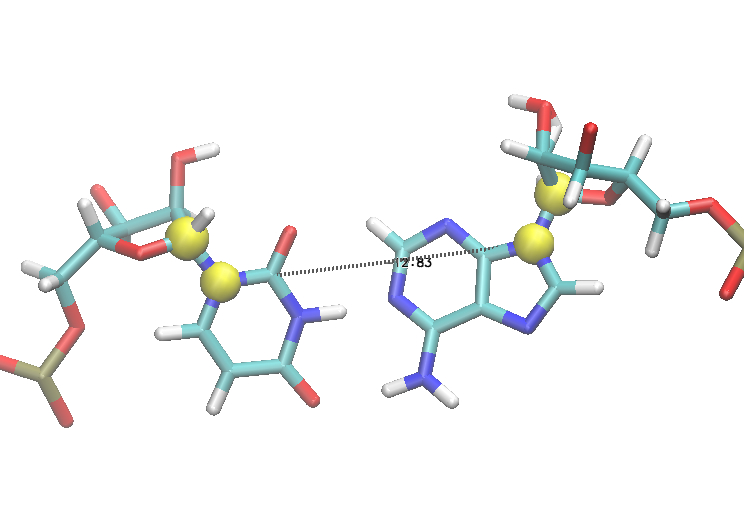
\includegraphics[width=5.5cm]{./pictures/torsion_angle_cis.jpg}}
\subfigure[Trans]{
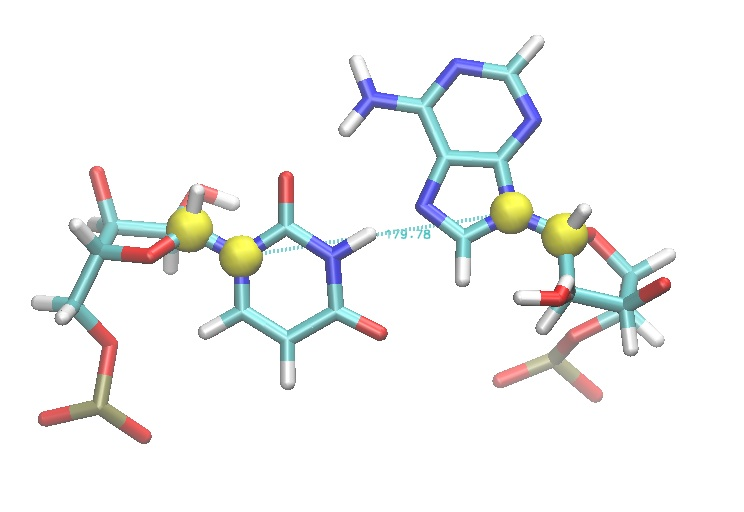
\includegraphics[width=5.5cm]{./pictures/torsion_angle_trans.jpg}}
\end{center}
\caption{Yellow spheres correspond to C1' and N1 atoms in pyrimidines and N9 atoms in purines. The torsion angle created by these four points determines the geometric isomerism of the two nucleotides creating a pair. }
\label{Conf}
\end{figure}

%Stacking interactions
\subsection{Stacking}
Stacking is an important non-covalent interaction contributing to the stability of both double helix and single stranded structures of nucleic acids \cite{Hobza2008}. It is suspected to be especially important for RNA molecules. In tRNA only a half of the nucleotides form a helix, but about 90\% of residues is stabilized by stacking \cite{Bloomfield1999}. 

\begin{figure} [h!]
\begin{center}
\subfigure[]{
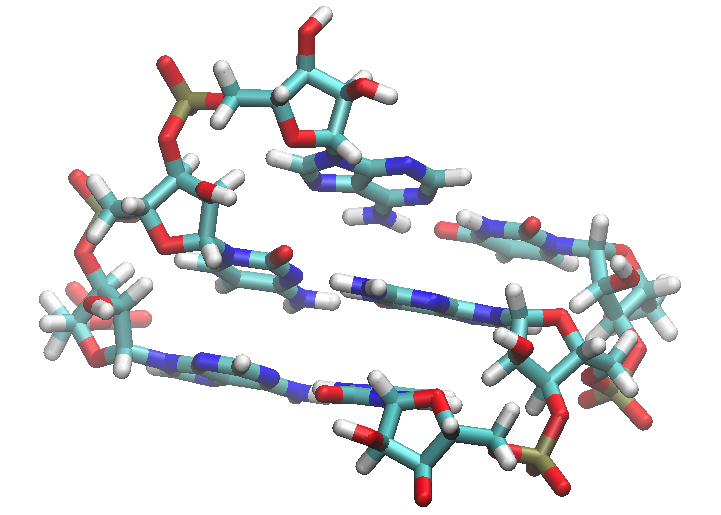
\includegraphics[width=5.0cm]{pictures/stacking1.png}}
\subfigure[]{
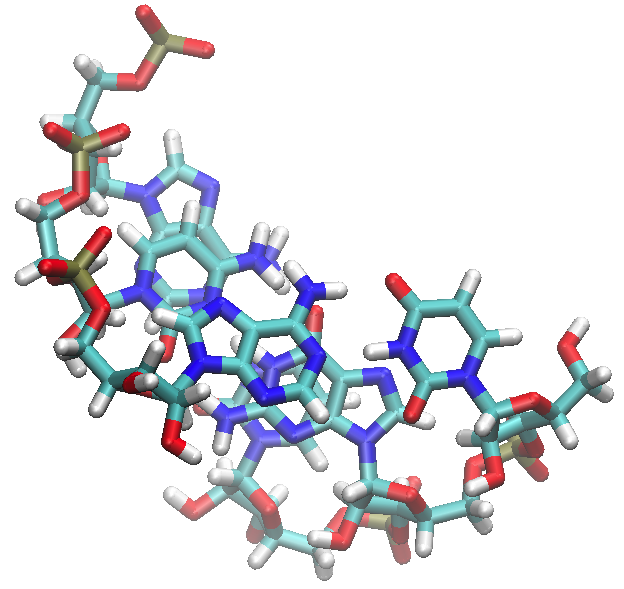
\includegraphics[width=5.0cm]{pictures/stacking2.png}}
\subfigure[]{
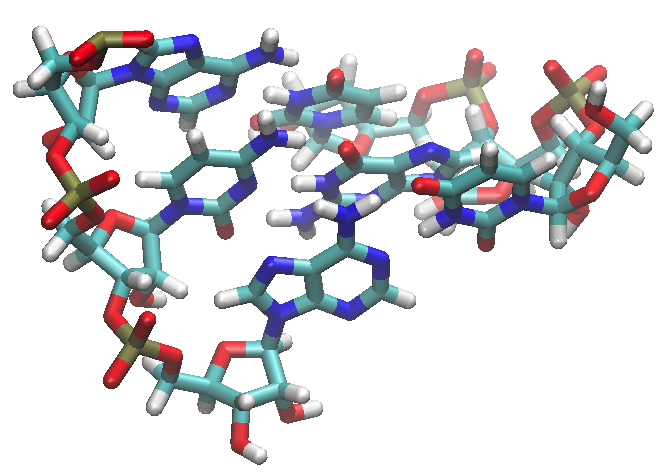
\includegraphics[width=5.0cm]{pictures/stacking3.png}}
\caption{Three-pairs of an RNA helix seen from different angles to expose  stacking between parallel bases.}
\label{StackingHelix}
\end{center}
\end{figure} 

Generally, stacking occurs between aromatic rings, in nucleic acids between the nucleobases. There is a general belief that the basis of stacking lies in the contact of the electron $\pi$-systems. Stacking is also supported by three phenomena: Van der Waals (dipole or induced-dipole attractions), electrostatic and solvation effects. It seems to be more important in folding of nucleic acids than proteins because nucleotide bases are more polarizable than most amino acids. 

%In order to measure stacking separately of hydrogen bonding the experiments where conducted with a helix terminated with a single nucleotide. Presence of the unpaired nucleotide  stabilizes the entire helix. Sites are uneven, for DNA the on the $5\prime$ site of the helix is more favorable energetically than the other one, but for RNA the $3\prime$ is \cite{Kool2001}. Experimental studies indicated ability of stacking among natural bases is the strongest between two purines, than purine-pyrimidine and pyrimidine-pyrimidine \cite{Guckian2010}.

We estimate stacking between two bases by calculating the energy of electrostatic ($U_{el}$) and Van der Waals ($U_{VDW}$) interactions applying the equations used in molecular mechanics:
\begin{equation}
U_{el} = k \sum{\frac{q_i q_j}{r_{ij}}}
\end{equation}

\begin{equation}
U_{VDW} = 4 \epsilon \sum{ \left[ \frac{1}{4} {\left( \frac{r_0}{r_{ij}} \right) }^{12} - \frac{1}{2} {\left( \frac{r_0}{r_{ij}} \right) }^{6} \right]}
\end{equation}
The sums consist of all pairs containing atoms from nucleobases $i$ and $j$. $k$ denotes the Coulomb constant ($k = \frac{1}{4 \Pi \epsilon_0}$), $q$ is the partial atomic charge of the atom, $r_{ij}$ is the distance between considered atoms, $\epsilon$ is the depth of the Lennard-Jones potential well for atoms $i$, $j$ and $r_0$ is the sum of Van der Waals (VDW) radius of atoms  $i$ and $j$.
We provide the VDW parameters and partial atomic charges from the Amber~\cite{Amber_ff} and Charmm~\cite{Charmm_2000_1, Charmm_2000_2} force fields. A set of parameters and charges may be also defined by the user in the file \texttt{charges\_andVDW.csv}. Only the nucleobases that are closer than the user defined cutoff (\texttt{cutoff\_stacking}) are considered in the stacking calculations. The unit for energy values obtained from described calculations is $kcal/mol$. 

It is believed that stacking is one of the best represented terms in molecular modeling. 
Especially with the Amber atomic charges which are fitted to molecular electrostatic potentials~\cite{Hobza2008a}. It was shown that calculations using the empirical potentials consisting of the Lennard-Jones VDW and Coulombic terms with atom-centered point charges were able to reproduce the {\it ab initio} stacking energy over the major portion of the conformational space~\cite{Leszczynski2002}.
\v{S}poner et al. in multiple works~\cite{Sponer1, Sponer_2, Sponer_3, Sponer_4} compared {\it ab initio} energies for about 300 geometries of stacked base dimers with data obtained by using empirical potentials. The agreement between these methods is remarkable, which suggests that calculations based on empirical potentials provide an excellent approximation of the stacking interaction energy between nucleotides. 


The electrostatic term, depending on the orientation of bases' dipole moments, may be attractive or repulsive regardless the bases are parallel or not to each other. While the VDW energy component is almost always favorable regardless base orientation.
What is more, the shape of nucleotides and method used for calculation the VDW energy, ensure that the lowest VDW values are obtained for parallel nucleotides which the biggest overlap.
It was also visible in our test calculations.
Thus we recognize two nucleotides as stacked, if their VDW energy is lower than \texttt{vdw\_cutoff\_stacking} parameter. 
The default value is $ -0.5 kcal/mol$.
It was found by trial and error and seems to be appropriate for the nonmodified nucleobases.


%\subsection{Anion-$\pi$ contacts} Following recent research on the types of non-covalent contacts in RNA molecules, \texttt{MINT} also analyzes the anion-$\pi$ - contacts and hydrogen bonding interactions, per nucleotides and in pairs \cite{Auffinger2013}. Detection of these interactions is based on the distance between the oxygen atom and the center of the mass of a nucleobase ring. 

\subsection{Ion-$\Pi$ interaction}
In biomolecules such as RNA, proteins and their complexes the non-covalent interactions play significant role. Hydrogen bonds are the most known non-covalent interactions but not the only one. For example the cation-$\Pi$ interactions, namely the non-covalent bonding between a monopole (cation) and a quadrupole ($\Pi$ system), seems to play important role in proteins structure.
Similar interaction was reported for the RNA molecules, but it was found that nucleic acid aromatic systems prefer to interact with anionic rather than cationic species~\cite{Auffinger_davos}. 
MINT allows to search for anion-$\Pi$ interactions involving RNA backbone phosphate groups and nucleotides bases. The example is shown in Figure \ref{stackingPiExamples}.
\begin{figure}[h!]
\begin{center}
\subfigure[]{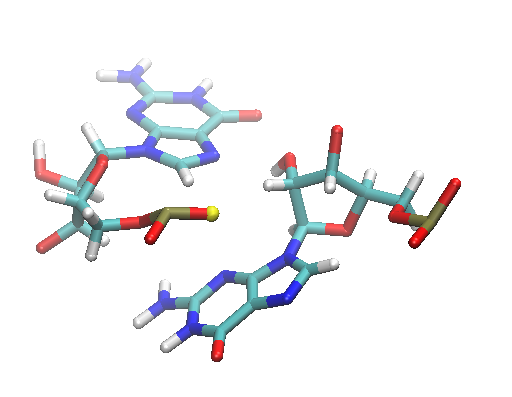
\includegraphics[scale = 0.3]{pictures/stacking_pi_1.png}
\label{stackingPiexample1}}
\subfigure[]{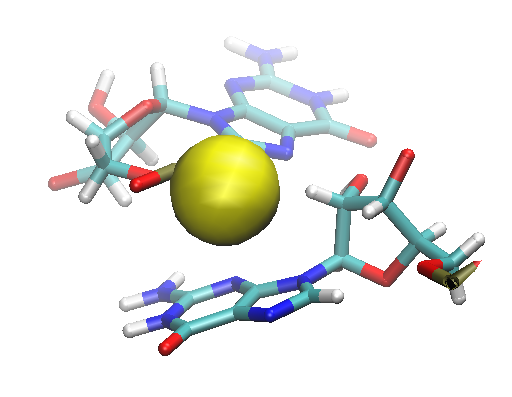
\includegraphics[scale = 0.3]{pictures/stacking_pi_2.png}
\label{stackingPiexample2}}
\subfigure[]{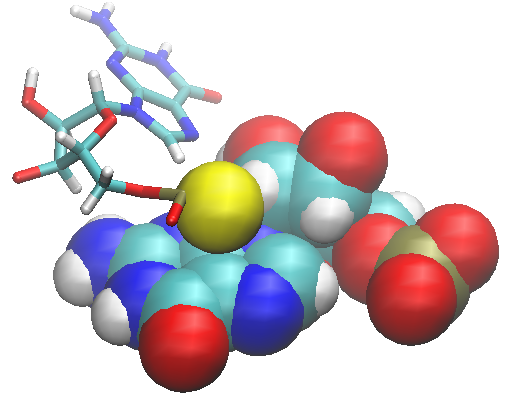
\includegraphics[scale = 0.3]{pictures/stacking_pi_3.png}
\label{stackingPiexample3}}
\caption{Three representations of the oxygen atom (yellow) "stacking" over the guanine base. The yellow sphere in the \label{stackingPiexample1} picture corresponds to the real VDW radius.}
\label{stackingPiExamples}
\end{center}
\end{figure}
Potentially interacting systems are recognized by distance criterium and than energy of interaction between phosphate atom and nucleotide base is calculated in the same way as in the stacking. 

\subsection{Representation of the RNA motifs}
Having all Watson-Crick pairs, a list-representation of the RNA secondary structure is created. We assume that one nucleotide can have only one Watson-Crick partner. If the second WCWC partner is encountered, all three nucleotides are denoted as a triplex. The index of the list represents the nucleotide number; the stored value is the index of its Watson-Crick partner. The list is easy-interpretable when the arcs connecting the pairs are drawn as  presented in Figure \ref{SecondaryStructureList}. 

\begin{figure}[h!]
\centering
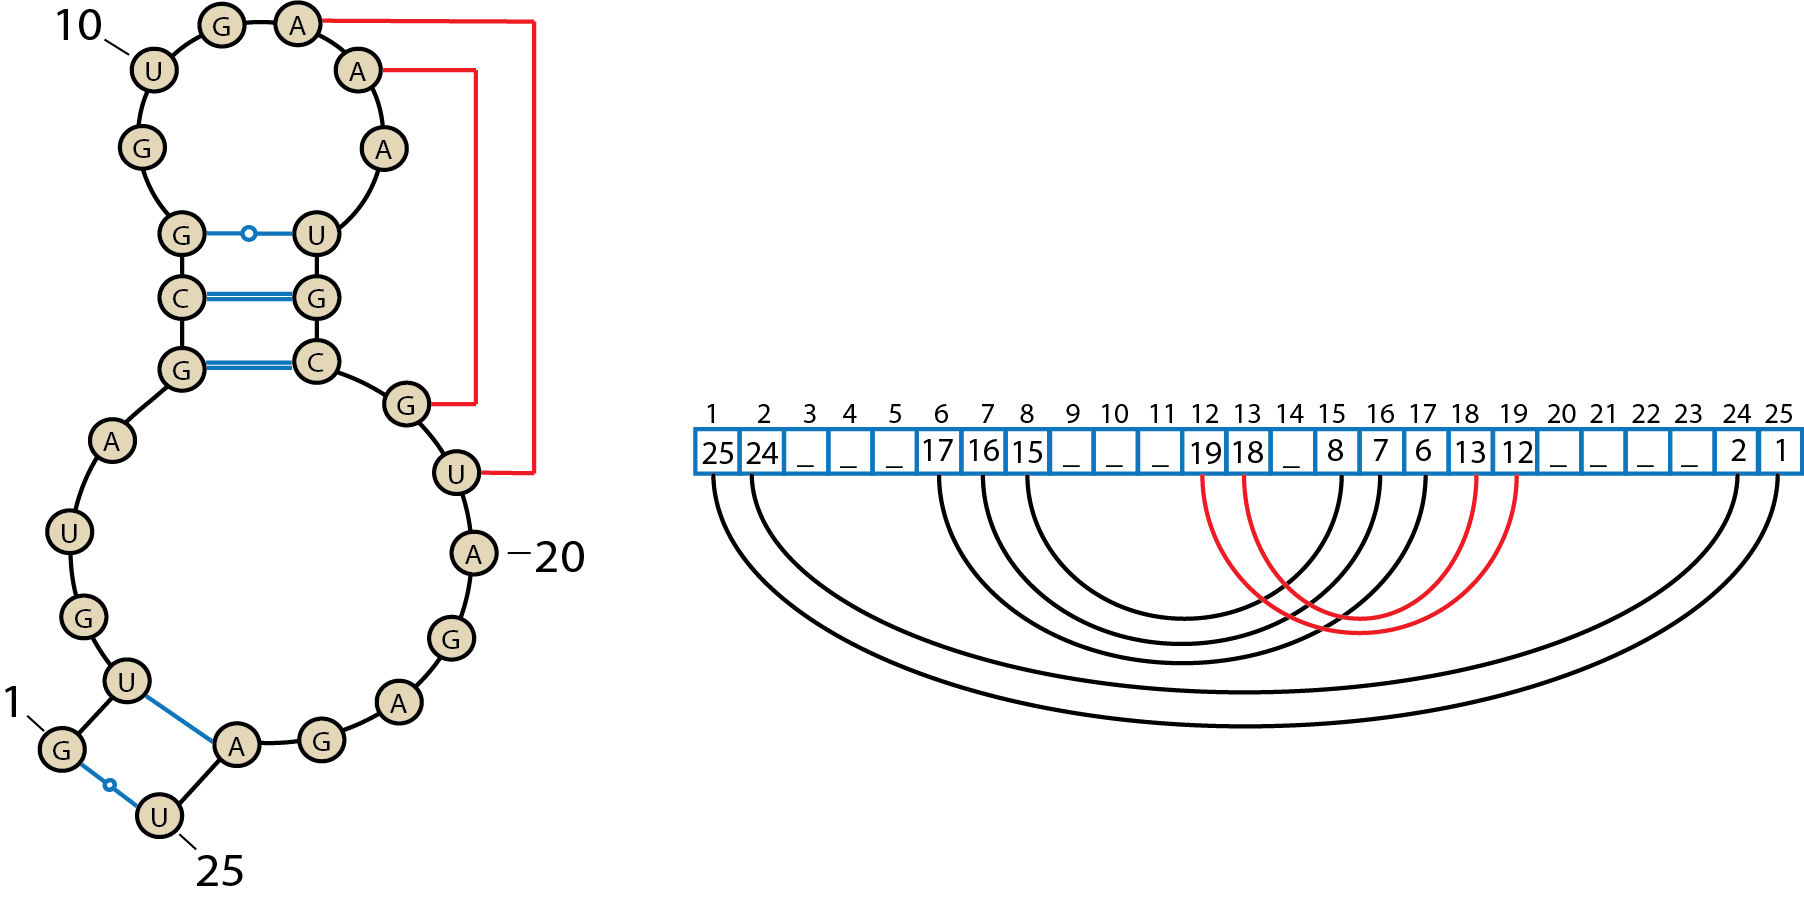
\includegraphics[width = \textwidth]{./pictures/PseudoKnotArchs.png}
\caption{Secondary structure of an exemplary RNA molecule and its list-representation. Red lines correspond to the Watson-Crick interactions creating a pseudo-knot.}
\label{SecondaryStructureList}
\end{figure}

\paragraph{Pseudo knots}
The list-representation contains also the information about the non-secondary motifs. The pseudo-knot is formed by the Watson-Crick interactions but creates three-dimensional folds as shown in Figure \ref{PseudoKnot}. Our program detects the pseudo-knot fold when the arcs intersect. A pseudo-knot is a symmetric structure -- both the three pairs 6--17, 7--16, 8--15  in Figure \ref{SecondaryStructureList} form the pseudo-knot as well as the two pairs: 12--19, 13--18. The natural way of solving this conflict is to choose the shorter list, in this case the pairs 12--19 and 13--18.  
\begin{figure}[h!]
\begin{center}
\subfigure[Tertiary structure]{
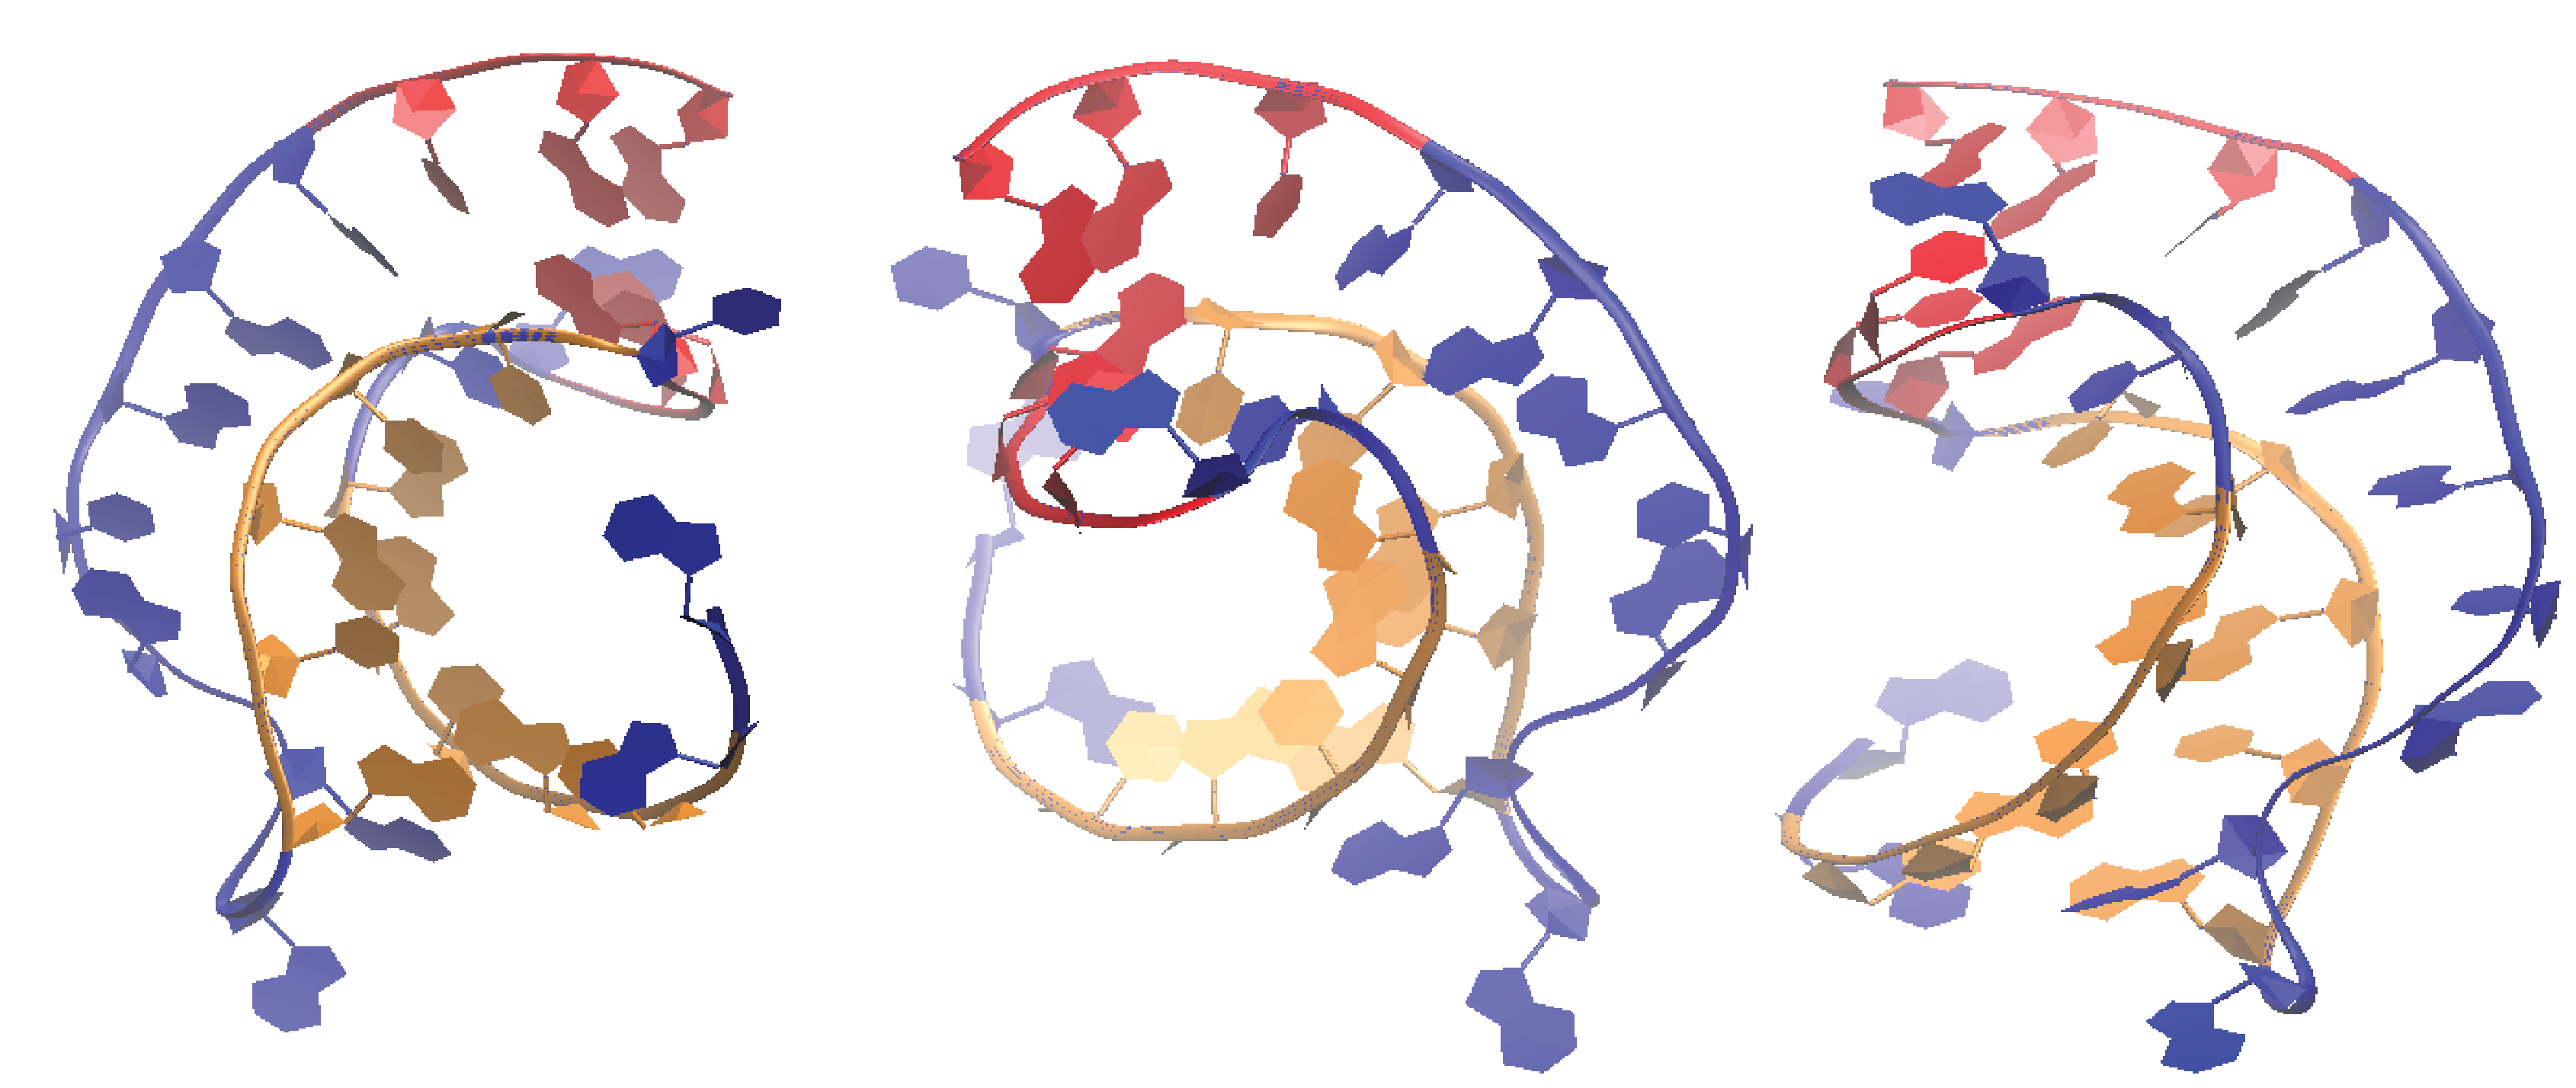
\includegraphics[width=12.5cm]{./pictures/pseudo_knot_combo.png}}
\subfigure[Secondary structure]{
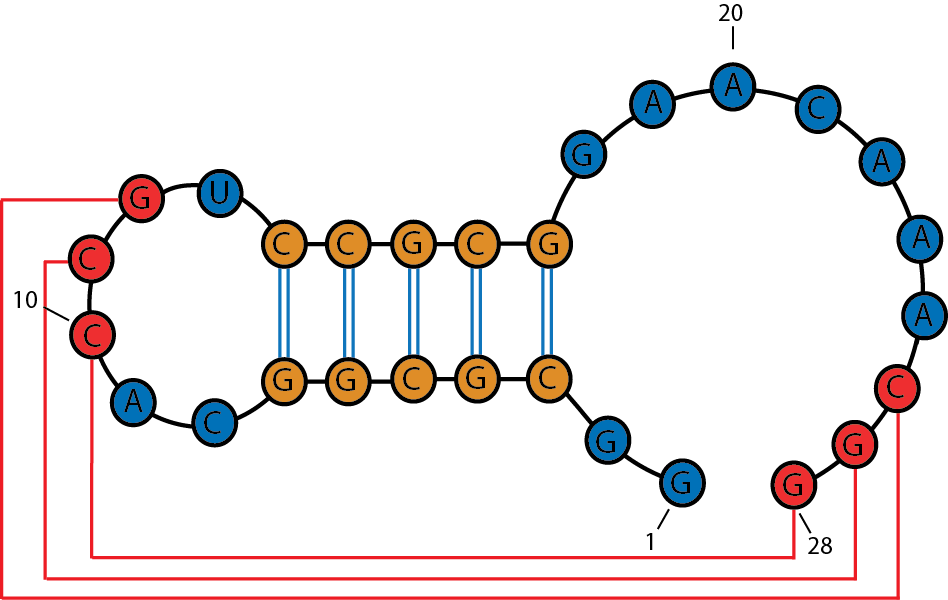
\includegraphics[width=6cm]{./pictures/pseudo_secondary_structure.png}}
\end{center}
\caption{An example of RNA structure with a pseudo-knot seen from three different angles. Nucleotides colored in red create a pseudo-knot, orange form a helix and blue refer to loops (PDB id: 437d).}
\label{PseudoKnot}
\end{figure}
\newpage
After detecting all pairs, and creating the list, the program finds all pseudo-knots and erases them from the list by putting the \texttt{None} value. Next, the program finds all kinds of motifs, that are defined as a set of unpaired nucleotides with the surrounding pairs as it is show in the figure \ref{MotifDesc}

\begin{figure}[h!]
\centering
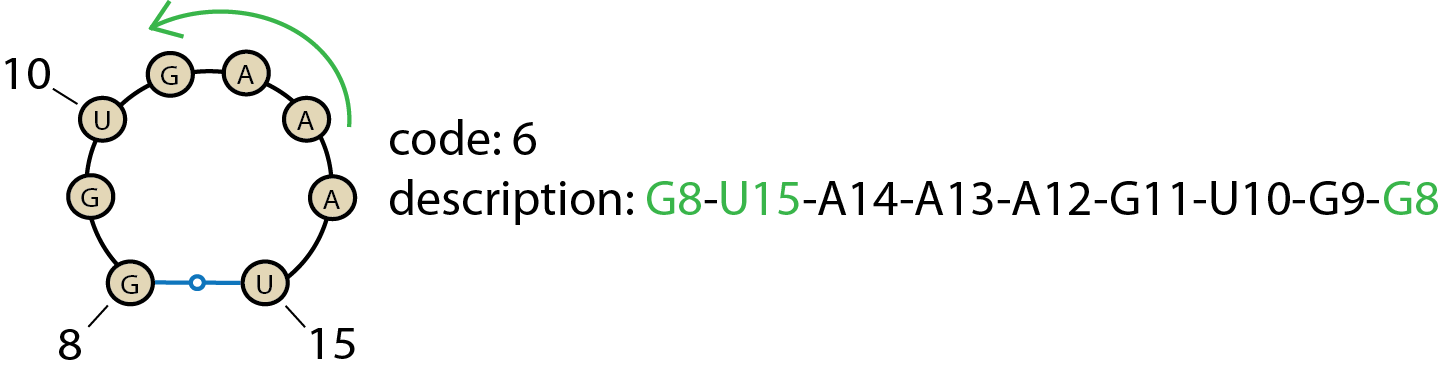
\includegraphics[width = \textwidth]{./pictures/motifs_description.png}
\caption{Program denotes the first pair (shown in green) and than list of unpaired nucleotides. Nucleotides are listed in accordance with the counter-clockwise direction.}
\label{MotifDesc}
\end{figure}

\begin{table}
\caption{RNA secondary structure motifs}
\label{RNAsecondaryStructures}
\begin{tabular}
{ >{\centering} p{5.5cm} >{\centering} p{5.5cm} >{\centering} p{5.5cm}}
&& \tabularnewline
 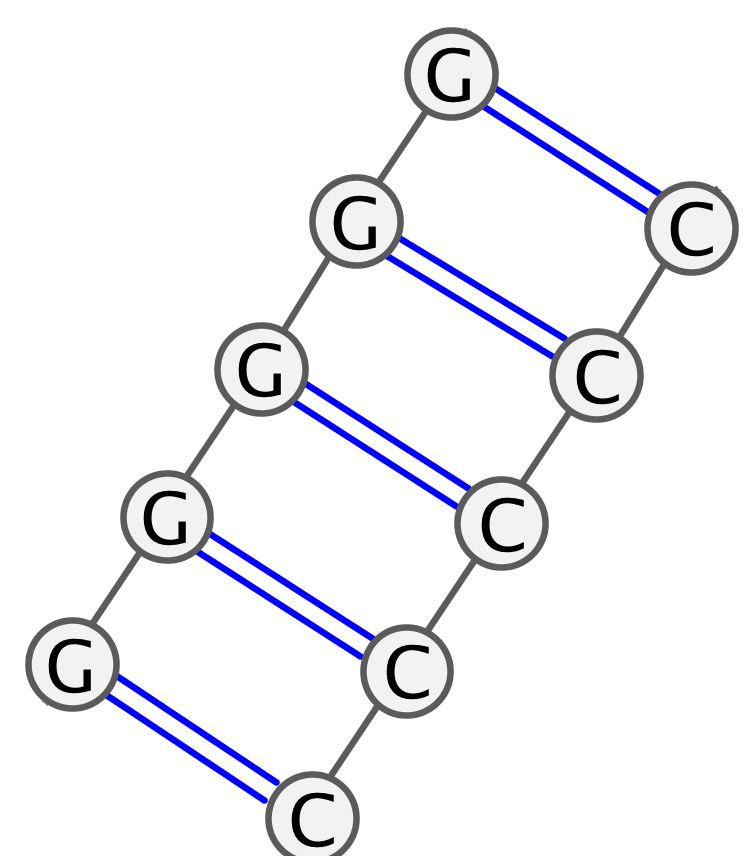
\includegraphics[width=4.5cm]{./pictures/helix_varna.PNG}  \linebreak Helix 
 & 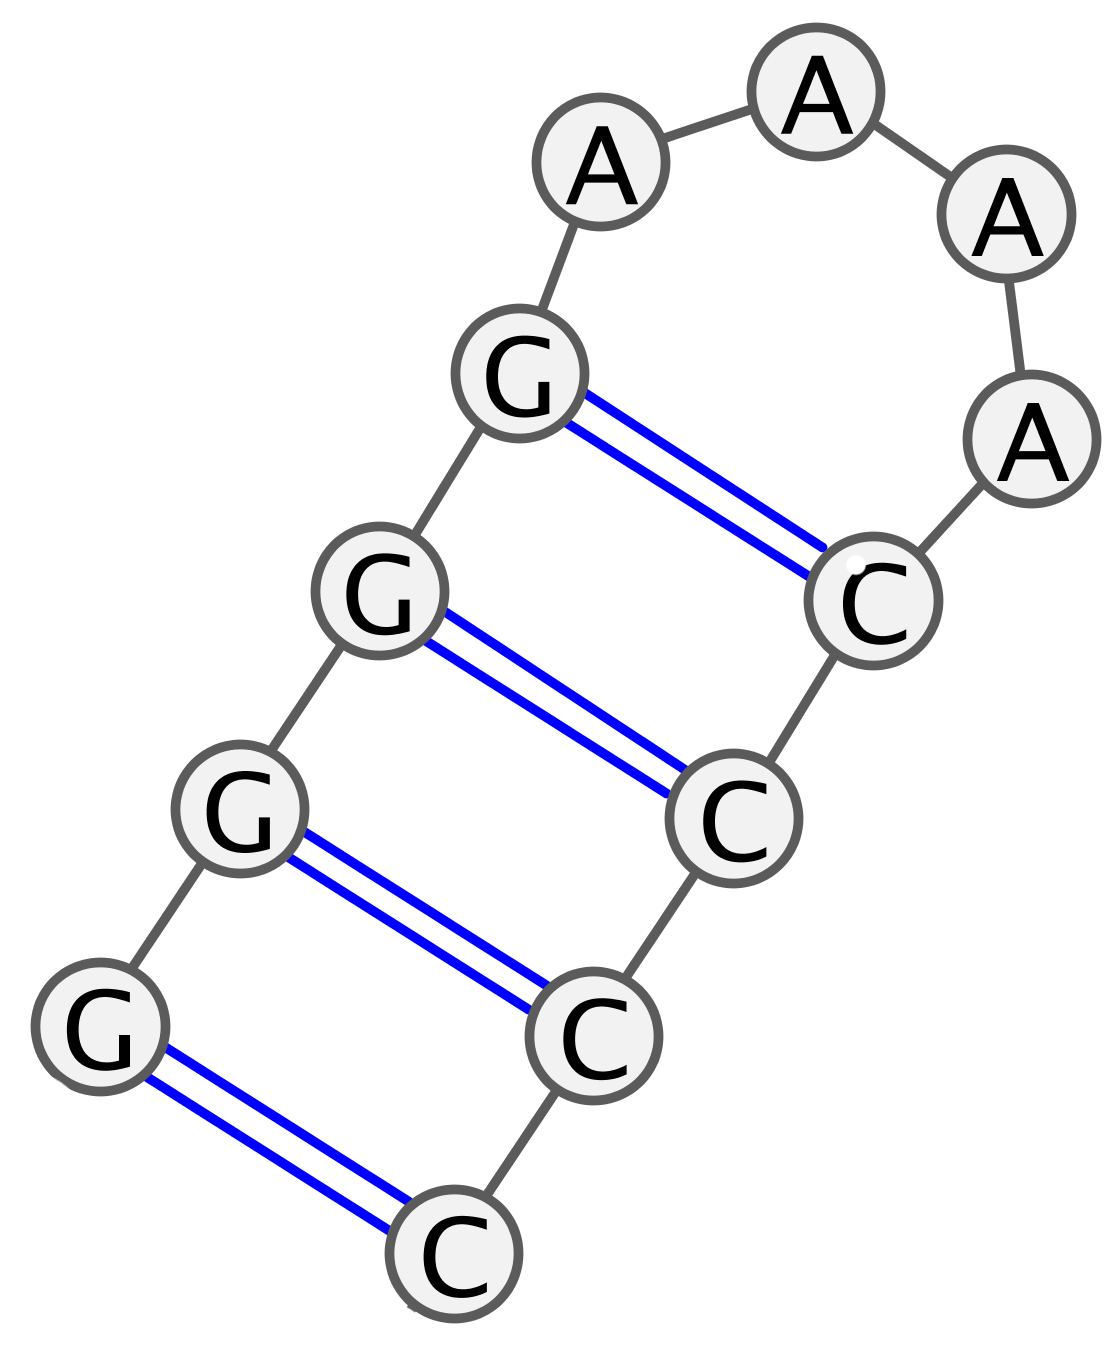
\includegraphics[width=4.5cm]{./pictures/hairpin_varna.PNG}  Hairpin loop \linebreak (code: 4) &  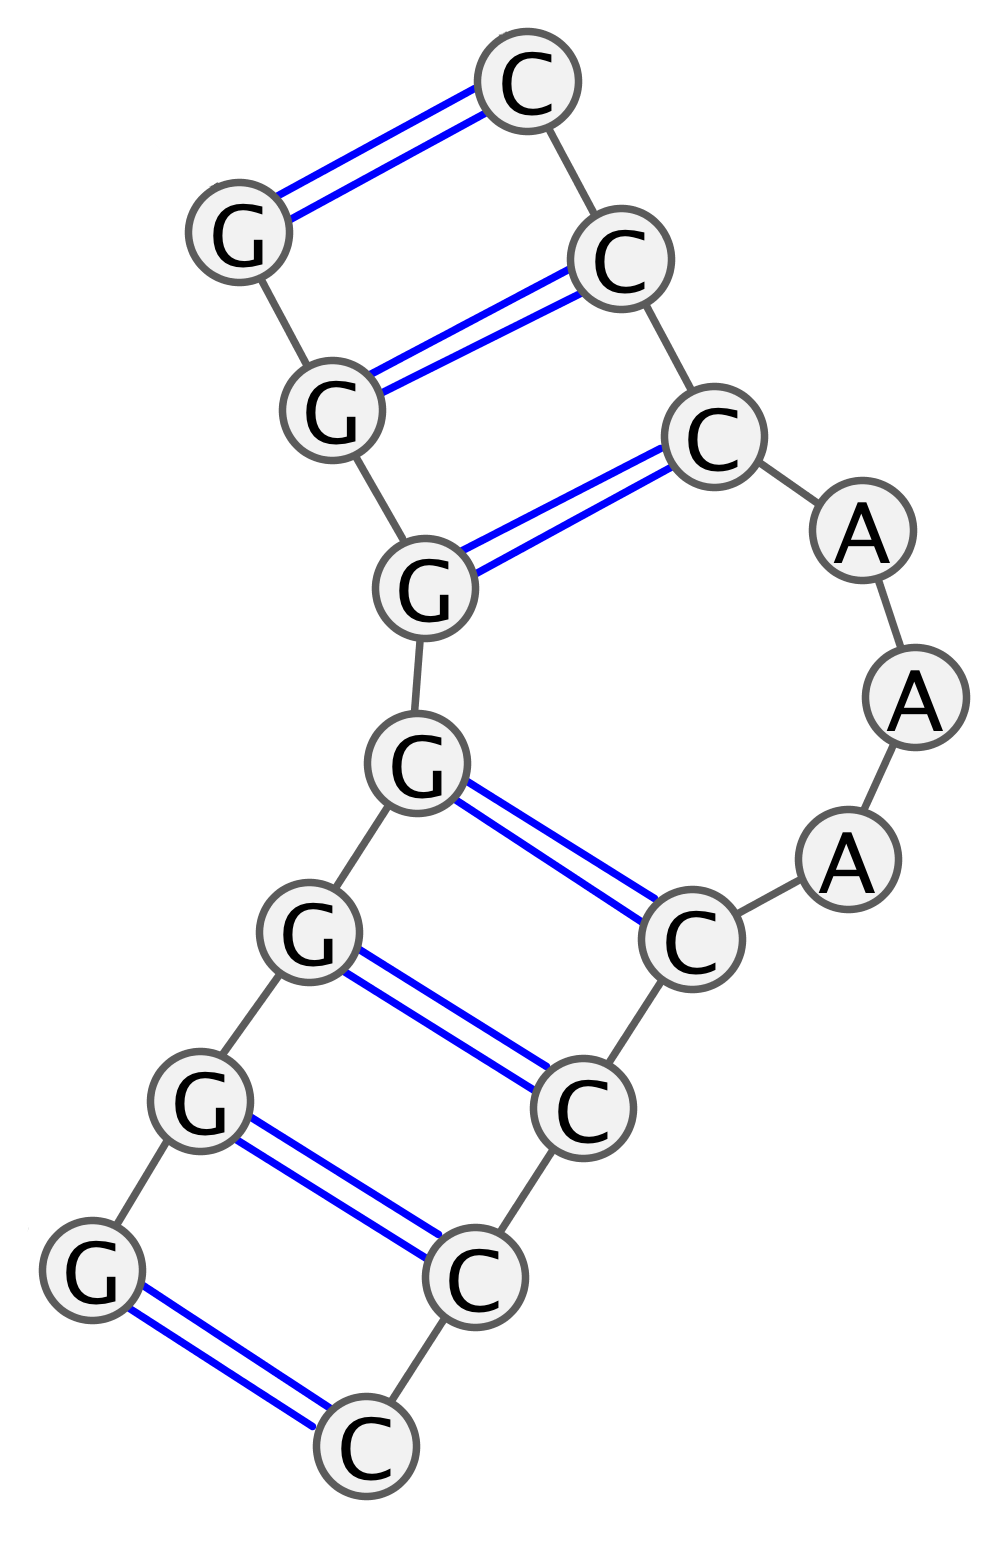
\includegraphics[width=4.5cm]{./pictures/bulge_varna.PNG} Bulge loop\linebreak  (code: 0--3) \tabularnewline
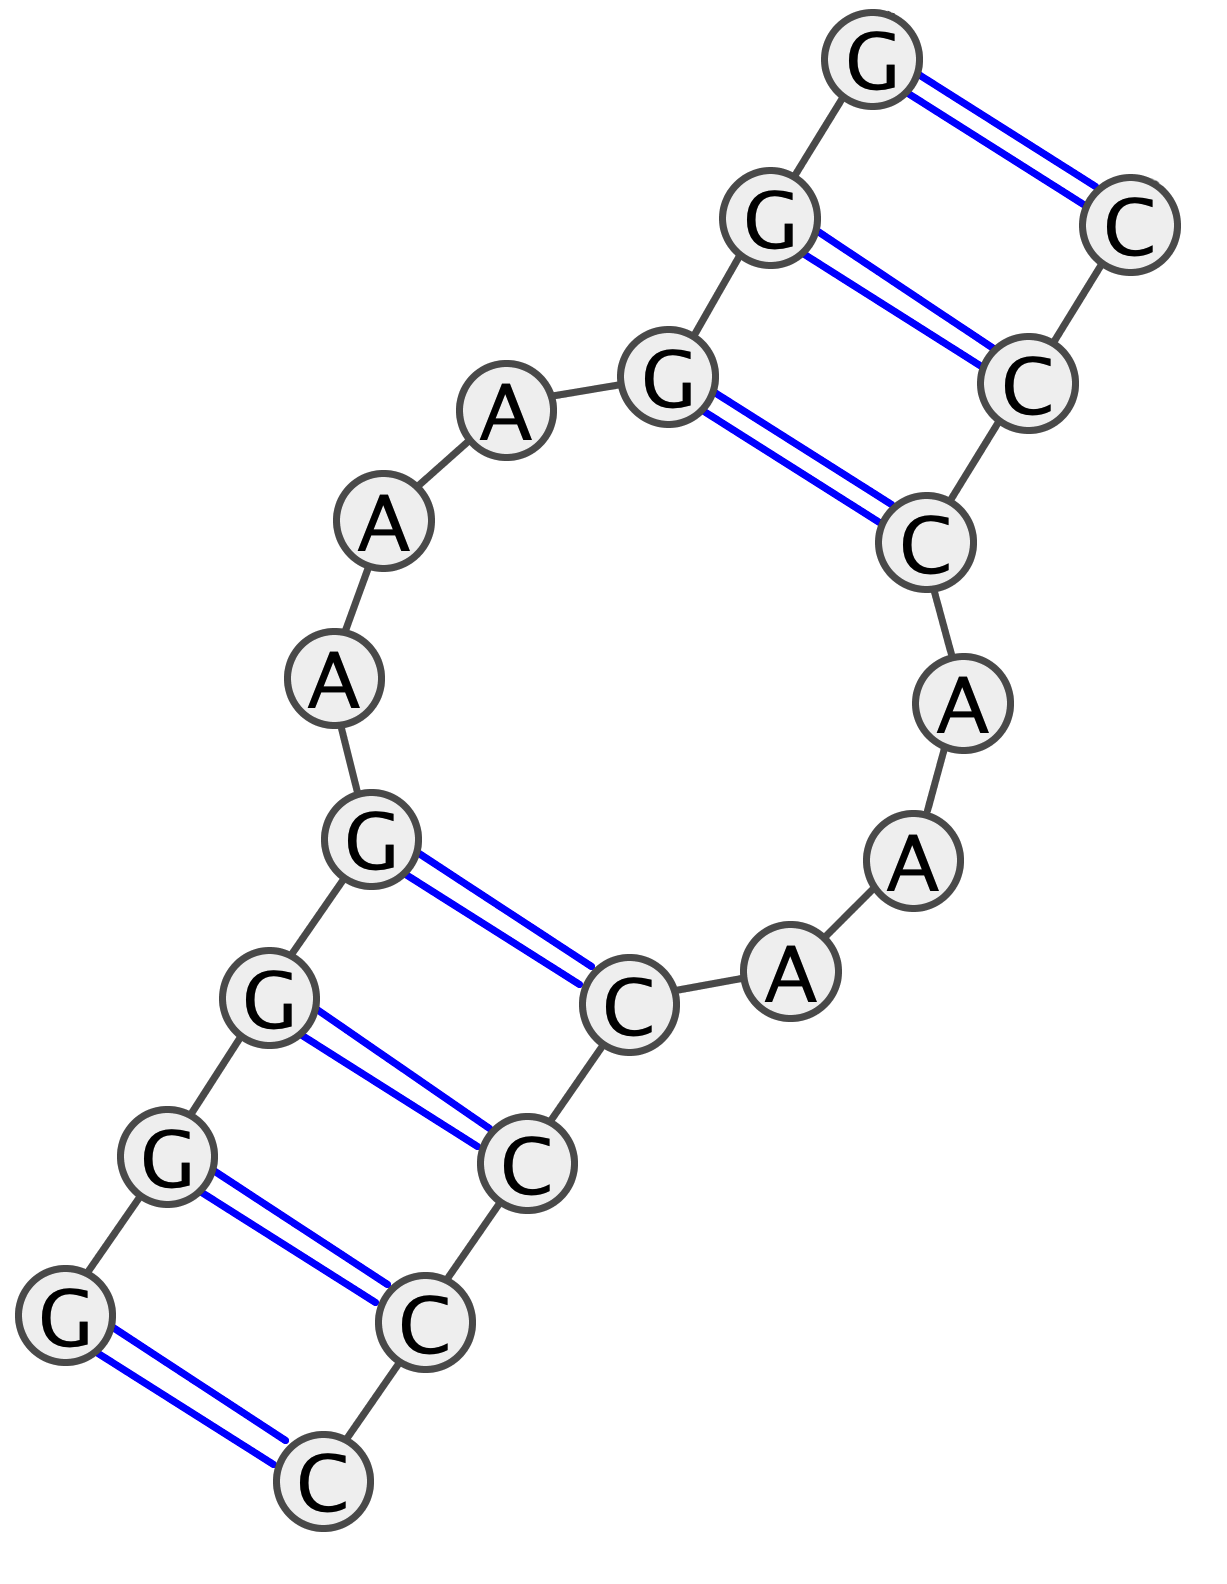
\includegraphics[width=5cm]{./pictures/interior_varna.PNG} Interior loop \linebreak  (code: 3--3) & 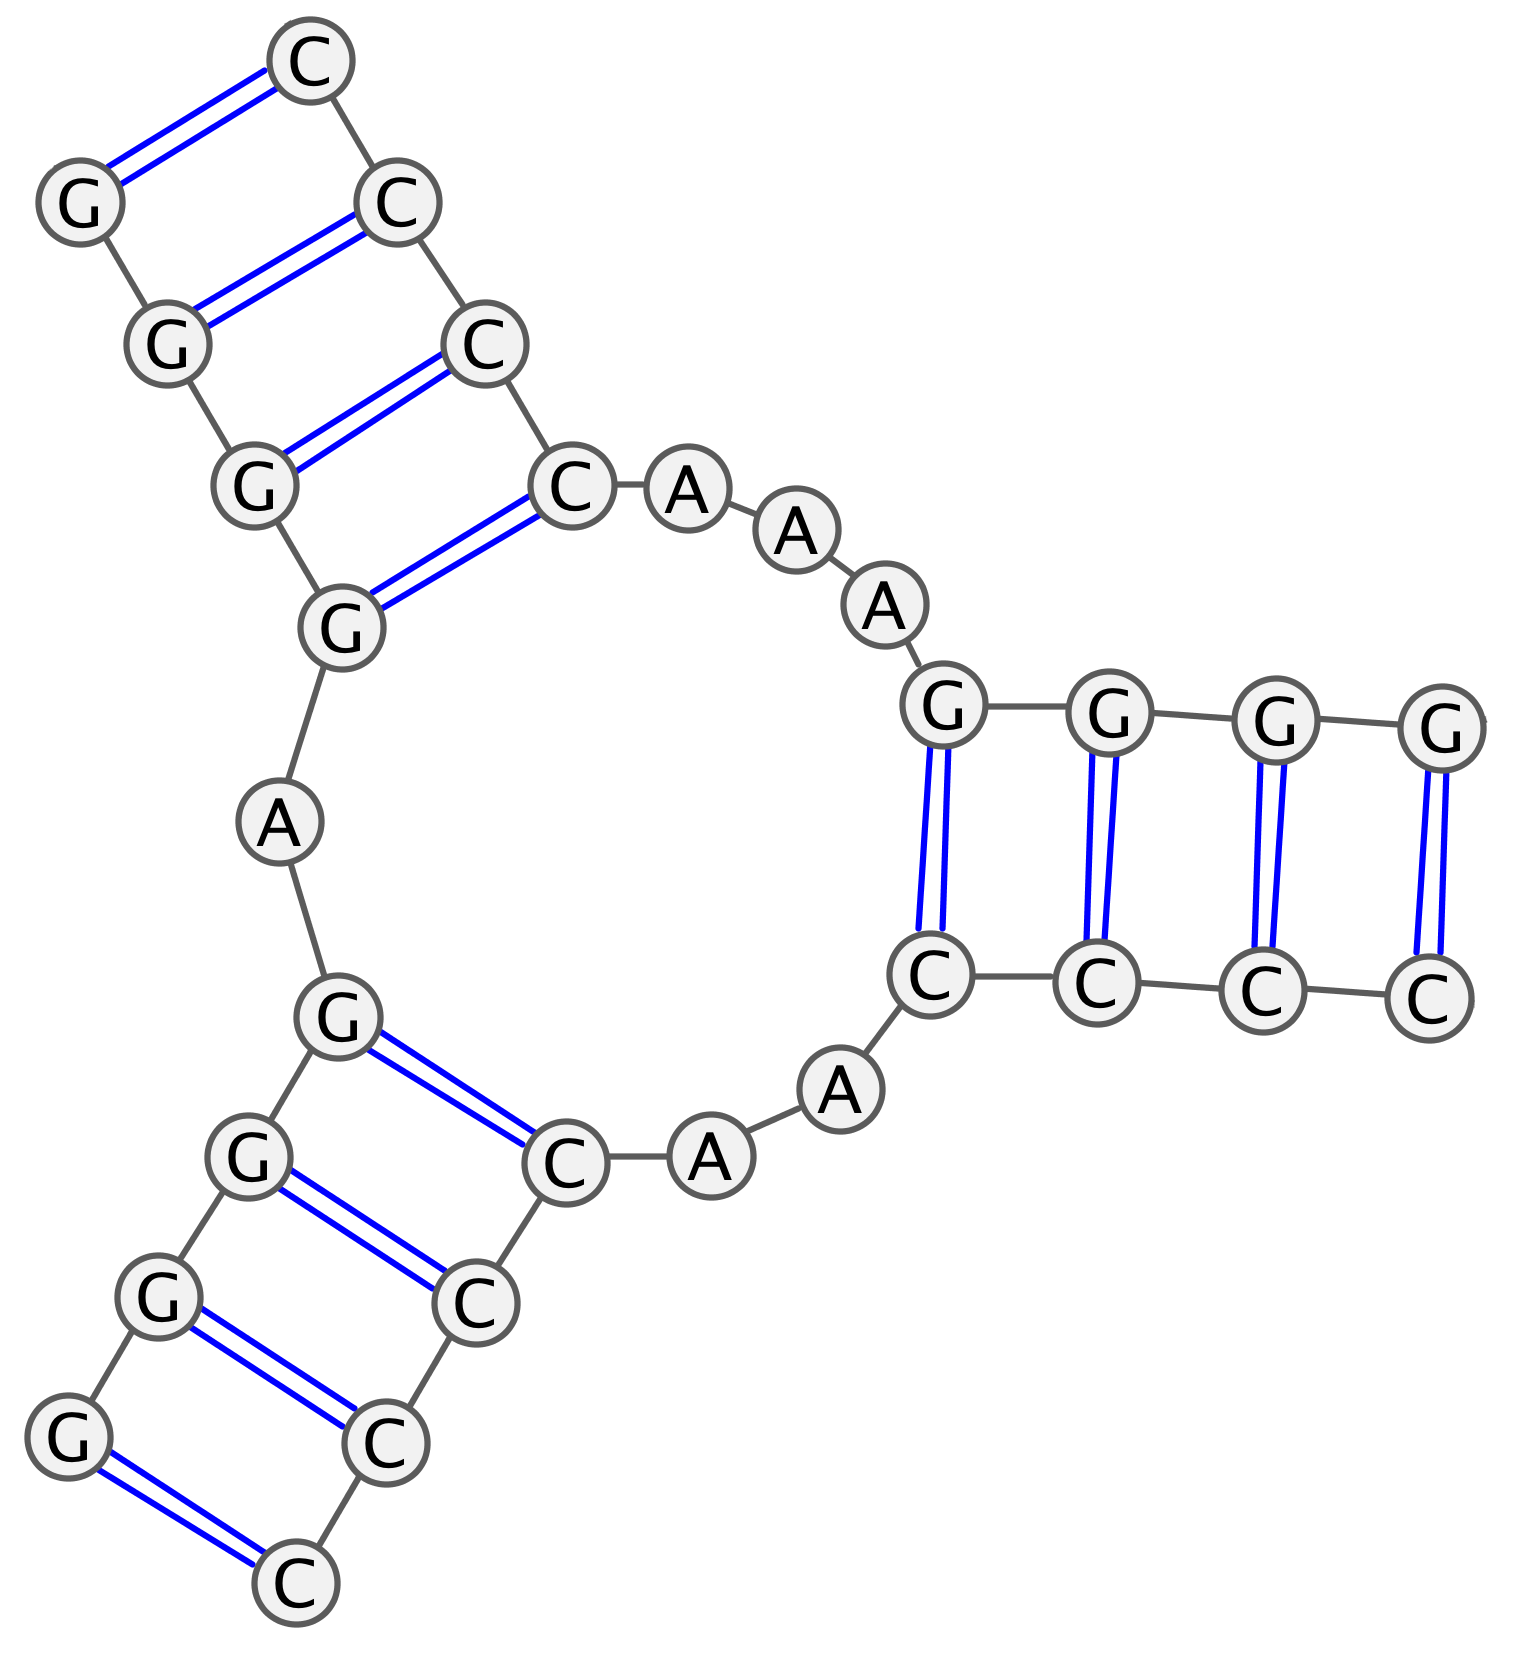
\includegraphics[width=5.5cm]{./pictures/multibranched_varna.PNG} Multi-branched loop\linebreak (code: 2--3--1) & 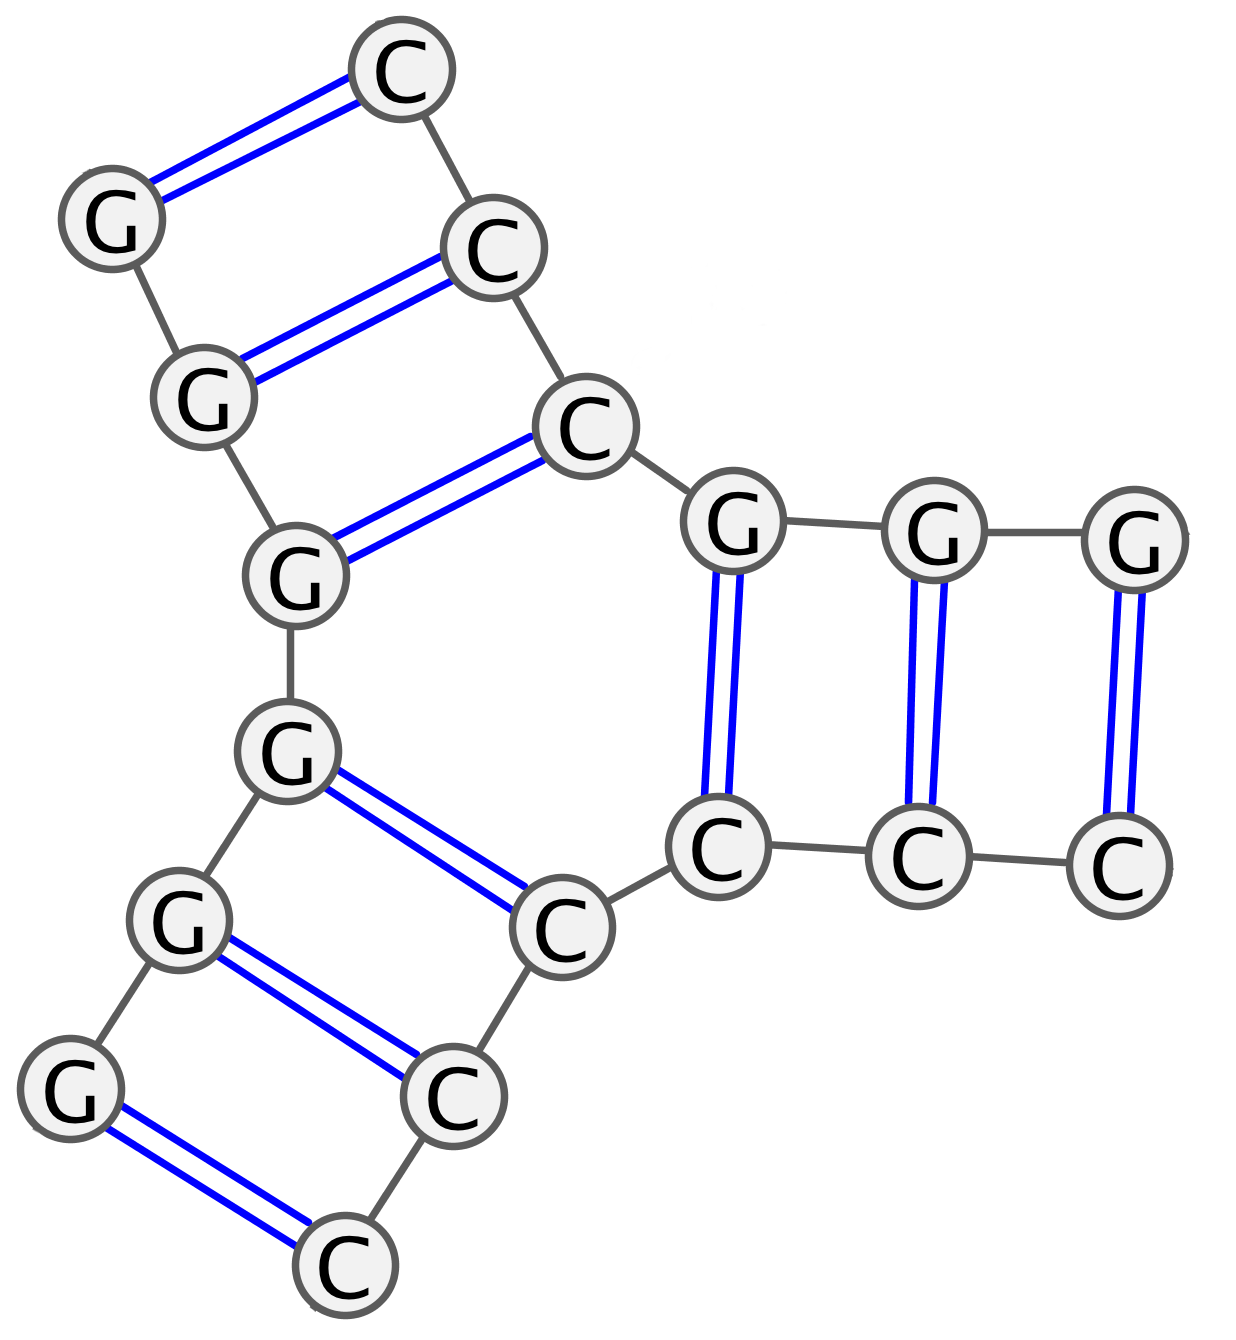
\includegraphics[width=5cm]{./pictures/junction_varna.PNG} 3-way junction\linebreak (code: 0--0--0)  \tabularnewline
&& \tabularnewline
\end{tabular}
\end{table}

\newpage

\paragraph{RNA motifs} nomenclature (loop, bulge, junction) can be inaccurate and misleading. The program uses the numerical description of the motifs that is understandable for people. The numbers correspond to the numbers of unpaired nucleotides between pairs. A four nucleotide loop at the end of a hairpin is represented by a single number 4. A symmetric bulge loop, with both bulges of the length of three is represented by two numbers: 3--3 and a three-way junction, without unpaired nucleotides is represented by three zeros: 0--0--0.  Different kinds of RNA secondary structure motifs are presented in Table \ref{RNAsecondaryStructures}. 

\subsection{Motif-search algorithm}
The algorithm uses a list representation of the RNA-secondary structure that contains the list of Watson-Crick pairs. As shown in Figure \ref{MotifsAlgorithm} the algorithm detecting helices and other secondary structure motifs walks through the list and stores the information about the visited nucleotides. As long as there are paired nucleotides it stores the information about the helix. When it encounters the end of the helix -- an unpaired nucleotide ahead of a pair, it starts to travel (search) around the motif. It stores the first pair as the beginning and goes to the index stored in the list. Then as long as there is an unpaired nucleotide it moves back -- with decreasing indices. When another pair is encountered, the algorithm goes into the indicated position and again moves back. The motif ends when the algorithm finds itself one step ahead of the starting index. The number of "jumps" is the number of values and the values represent the number of unpaired nucleotides in between. After one motif is found and classified, the algorithm jumps one step further than the last seen pair. The algorithm stops searching for the motifs and helices when the index is larger than the value stored in the list. 

\begin{figure}[h!]
\centering
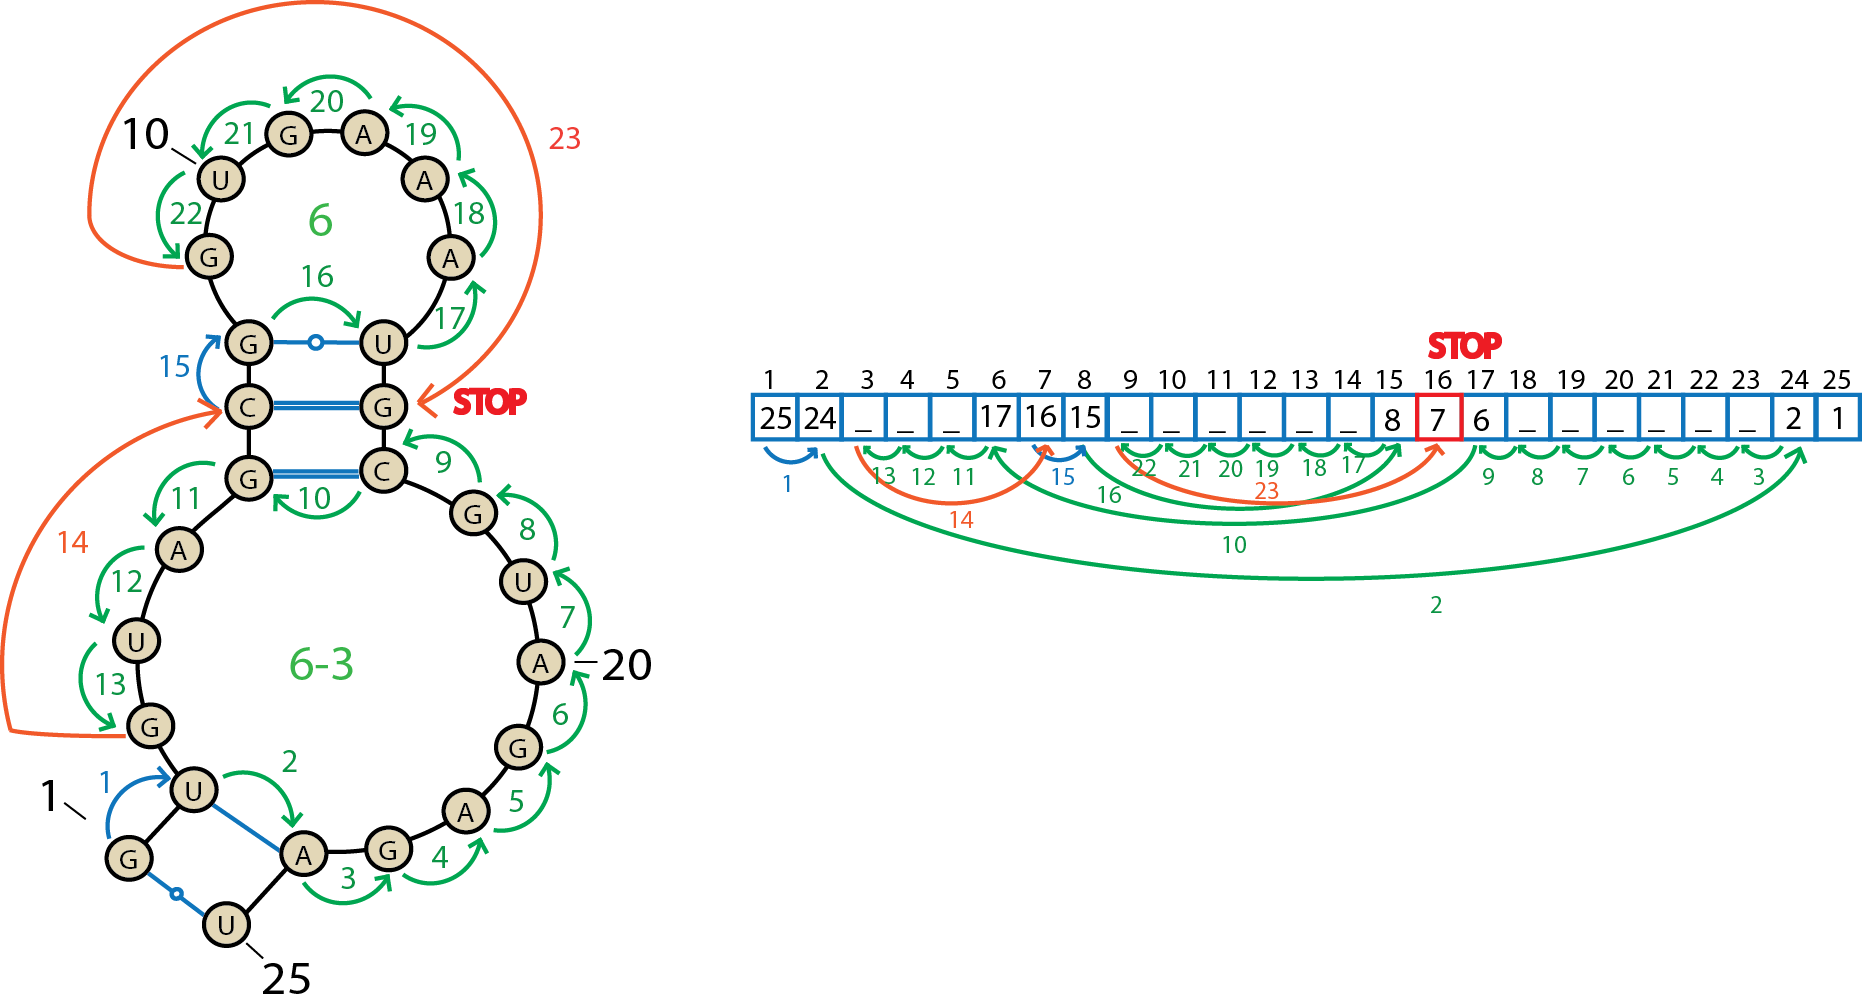
\includegraphics[width =\textwidth]{./pictures/algorithm.png}
\caption{Scheme presenting the steps of the algorithm that finds and classifies the motifs in the RNA structures. The numbers correspond to the step number. Green arrows correspond to the structural motif and blue to the helices. The orange lines denote the jumps after finishing the motif. The STOP sign indicates the position where the algorithm stops. }
\label{MotifsAlgorithm}
\end{figure}

As a result of the single frame analysis the program returns a list of all pairs, motifs and numerical characterization of all nucleotides. Every nucleotide is parametrized with the number of created hydrogen bonds and the description of its partner:

\begin{verbatim}
G538 , 538 , 3-C513A539:1 , 2-C513:2 , 3-C513:7
\end{verbatim}

First the type of the nucleobase with its PDB id, nex the PDB id one more time, and lists pairs the nucleotide created during the trajectory. Description of the configuration starts with the number of hydrogen bonds, than the nucleobase and PDB ID. There can be more than one nucleotide listed - what indicated the triplex. The number after a semicolon is the number of frames this pair or triplex were present.


\newpage

\section{Trajectory analysis}
If the case of a trajectory in which multiple RNA conformations have to be analyzed and classified, every frame is characterized in detail as previously described. The main output of the program is a set of \texttt{.csv} files listing all the pairs and motifs: helices, triplexes, pseudo-knots etc. and the number of the frames in which the considered structure was present, its topology and participating nucleotides. A detailed description of all the output files can be found in Section~\ref{OutputFiles}.

\subsection{Clustering}
To recognize and characterize the dynamics of the secondary structure of the RNA molecule, we have to cluster the detected secondary structure motifs. Clustering is parameterized with two user-defined parameters: \\
\begin{itemize}
\item \texttt{time\_cutoff} that defines the minimal percentage of frames in which the motif has to be present to be classified.
\item \texttt{margin} that defines the minimal percentage of similarities between the two motifs to belong to the common cluster. 
\end{itemize}

The fist step is to remove rare motifs (leaving only the significant ones) through their filtering according to the number of frames the motif appeared in. Below one can find an exemplary list of motifs after removing rare motifs:

\begin{figure}[h!]
\centering
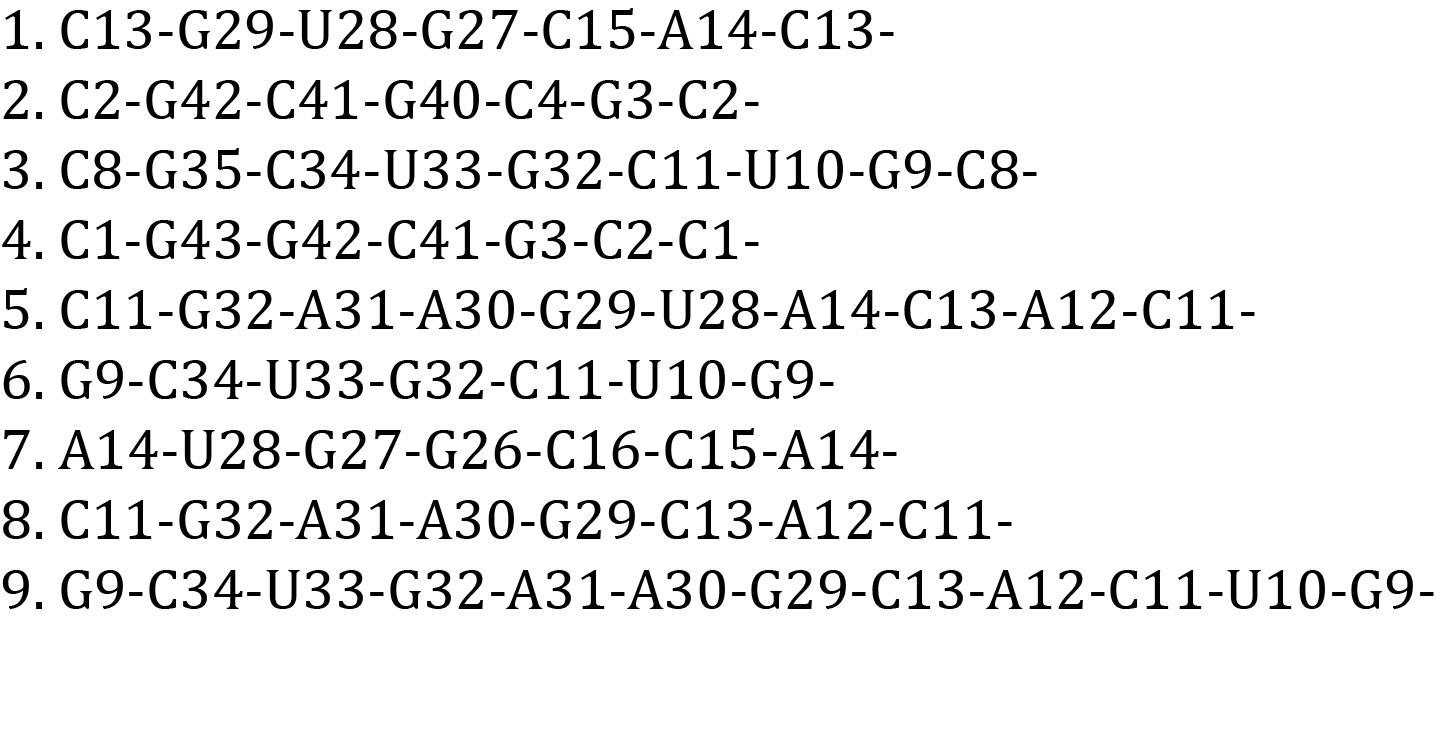
\includegraphics[scale=1]{./pictures/cluster_motif_step1.png}
\label{MotifsClusteringStep1}
\end{figure}

Next, the motifs distance matrix is computed. The distance between motifs is the number of their common nucleotides. The order of the nucleotides is not taken into account:
\begin{figure}[h!]
\centering
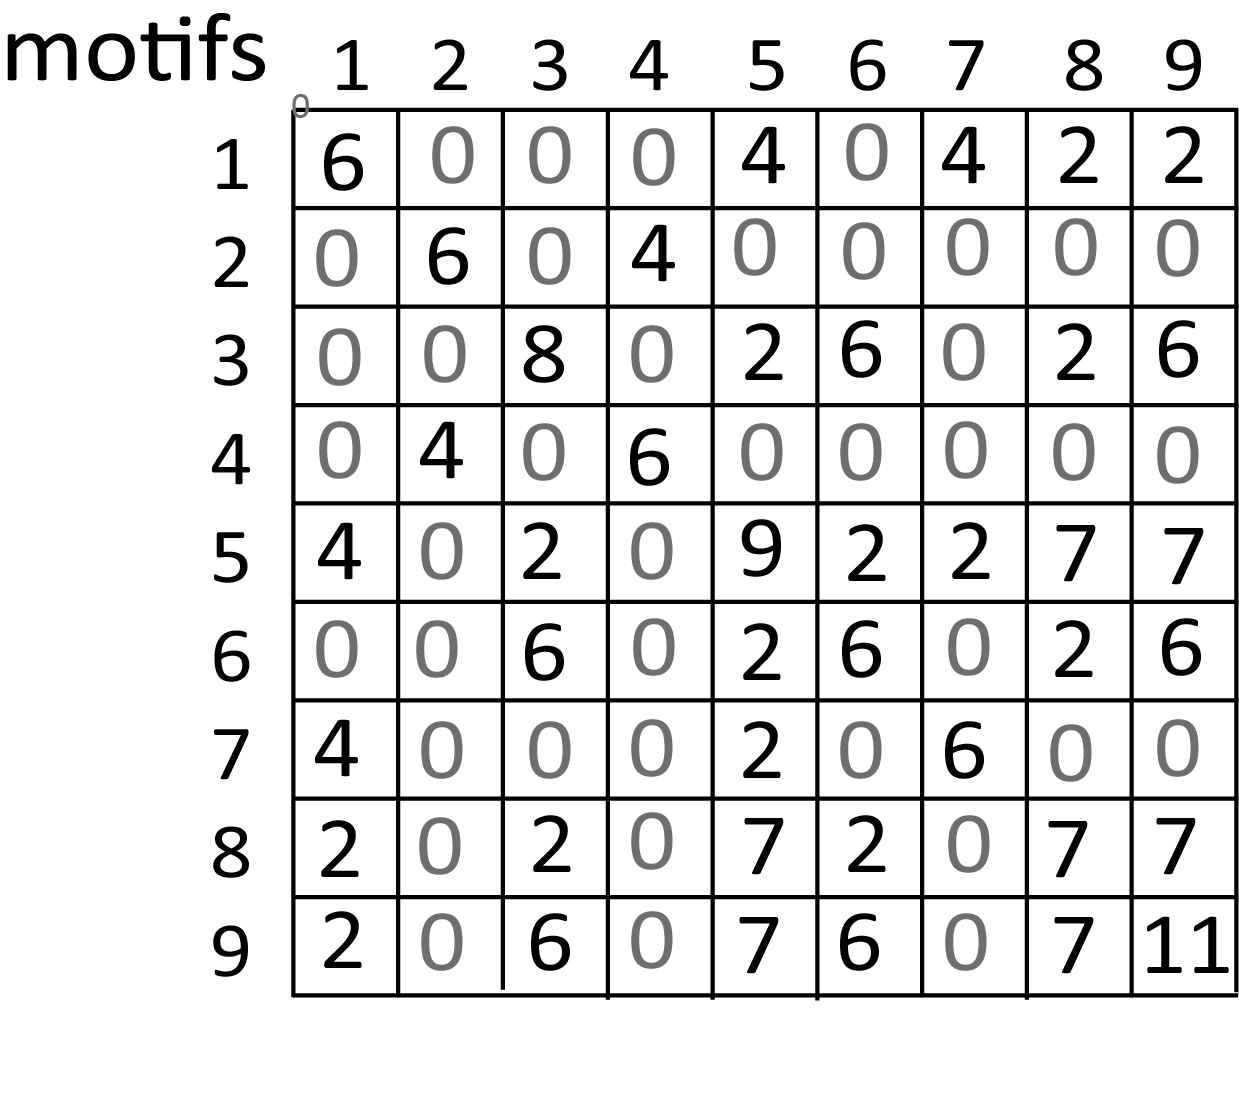
\includegraphics[scale=0.6]{./pictures/cluster_motif_step2.png}
\label{MotifsClusteringStep2}
\end{figure}

\newpage
Then, the partners for all motifs are denoted. The partner has to satisfy the distance requirement expressed by the equation shown below:
\begin{figure}[h!]
\centering
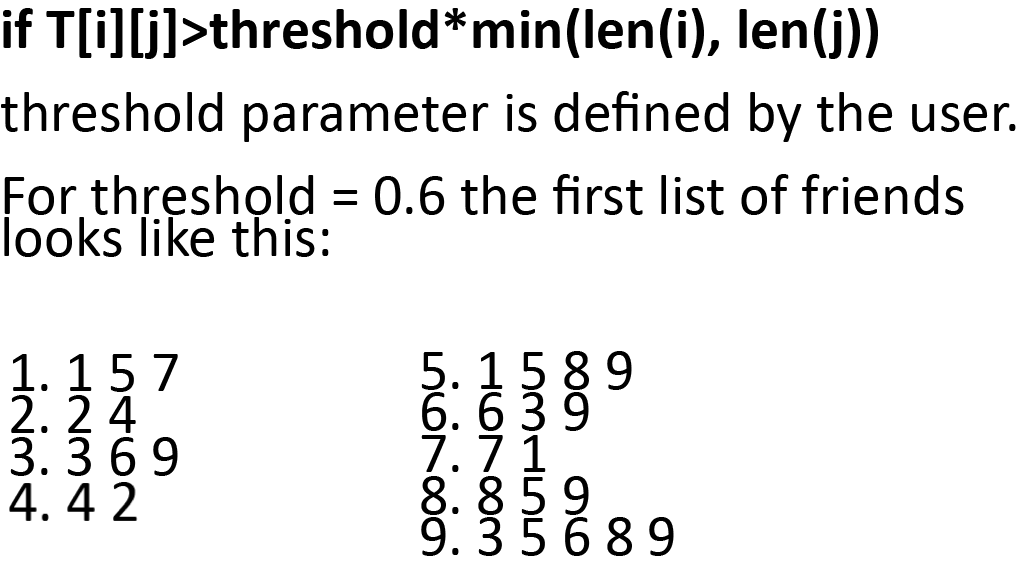
\includegraphics[scale=1]{./pictures/cluster_motif_step3.png}
\label{MotifsClusteringStep3}
\end{figure}

Next, the motif with the longest list of partners is incorporated as the first one to the first cluster number zero. The motifs used in the first cluster have to be crossed out from the rest. Then the second longer is chosen, the picked motifs are crossed out ant so on.  

\begin{figure}[h!]
\centering
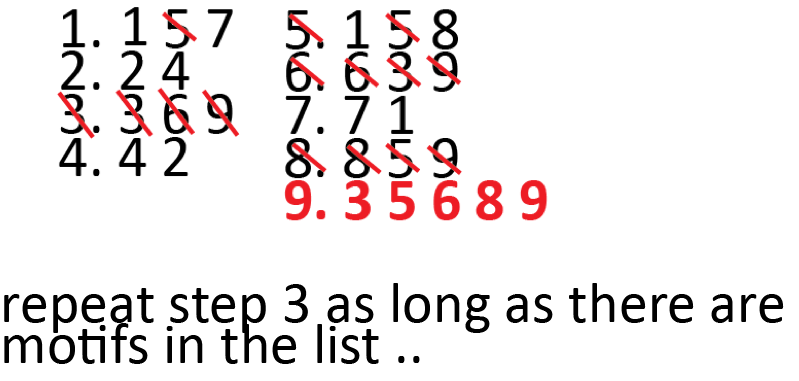
\includegraphics[scale=1]{./pictures/cluster_motif_step4.png}
\label{MotifsClusteringStep4}
\end{figure}

\begin{figure}[h!]
\centering
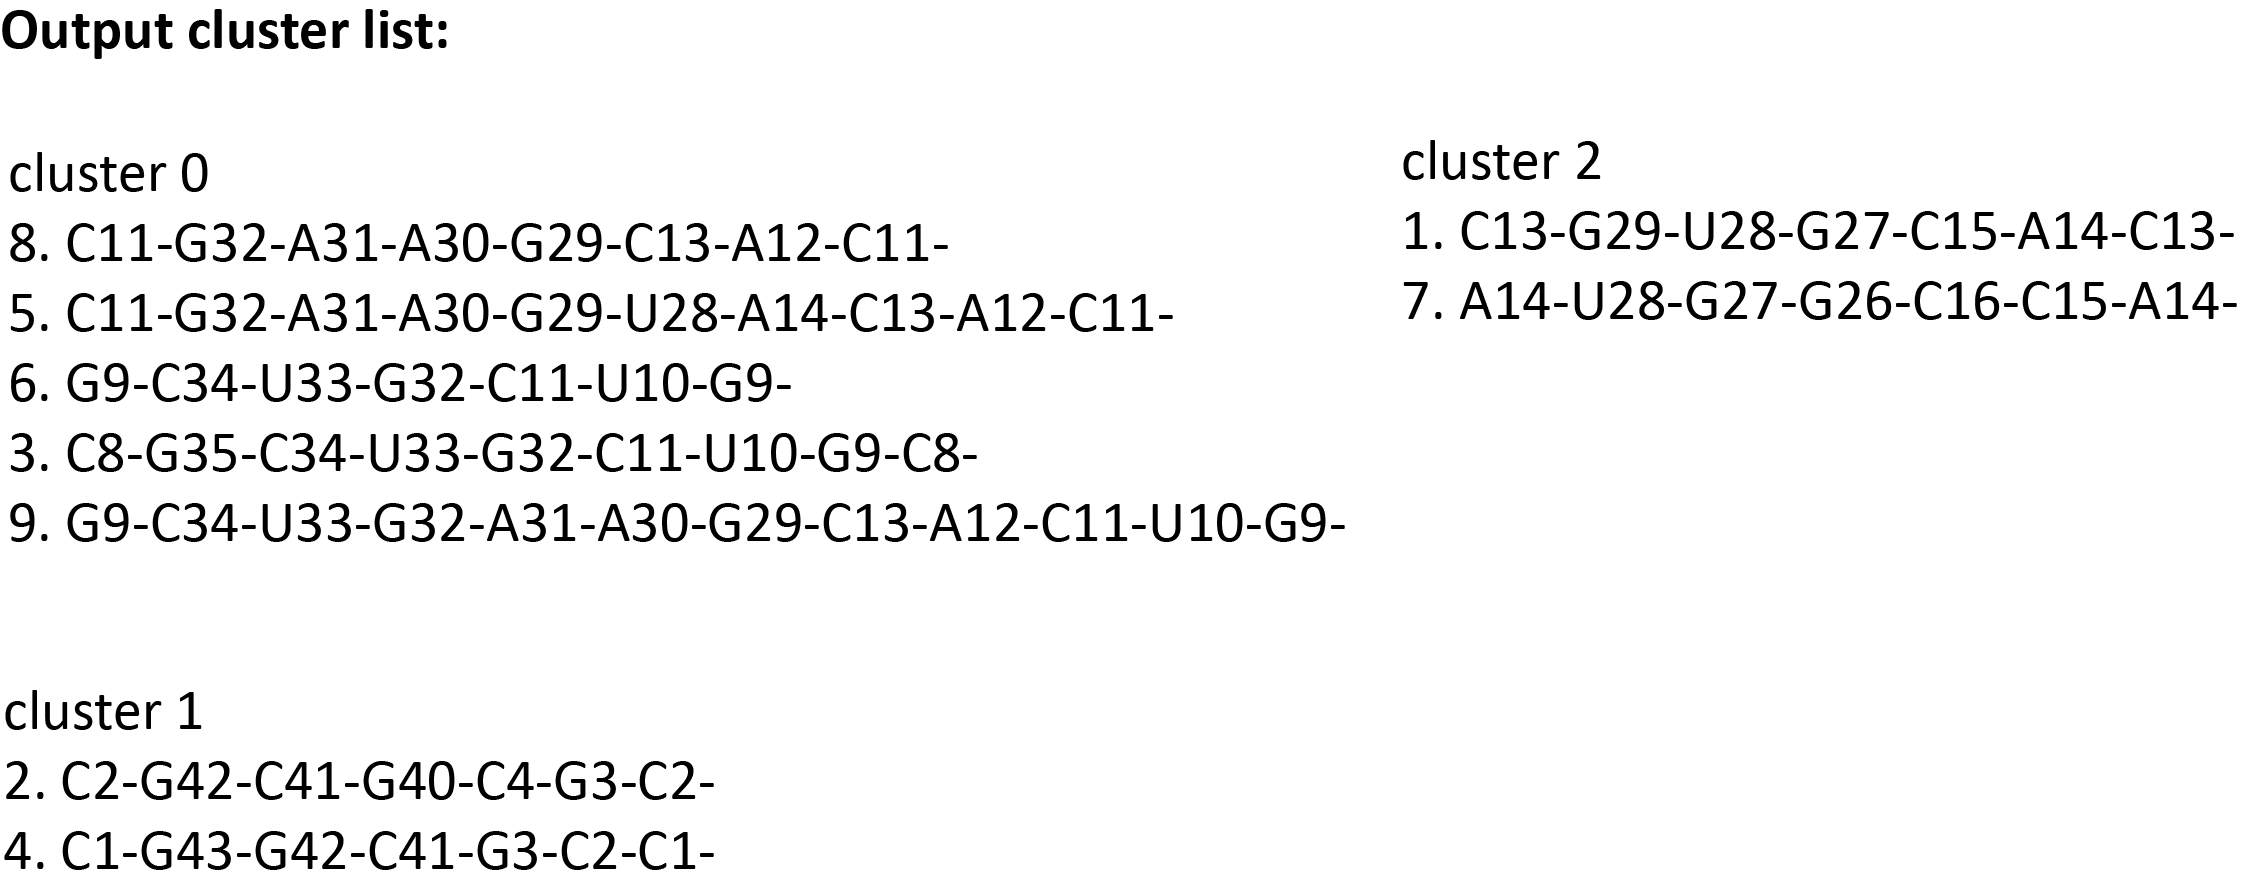
\includegraphics[scale=1]{./pictures/cluster_motif_step5.png}
\label{MotifsClusteringStep5}
\end{figure}

Additionally, the average clusters are returned. The list consists of the longest motif for every cluster and the two vectors of float values describing every nucleotide participating in the representative motif. The float vectors represent the average number of hydrogen bonds created by a nucleotide in both WC-WC pairs and other interactions. We hope to show the average secondary structure of the molecule within the tertiary structure description. While analyzing the whole output generated by the script, one can understand the complex description of the RNA structure in the dynamics.

\subsection{Parameters}
Parameters are stored in a dictionary that is an easy manageable structure set. The data are organized by keys; both the keys and their values can be of any type. Here, we describe the parameter dictionary \texttt{parms} which contains the keys that are text descriptors of the parameters:
\begin{itemize}
\item \texttt{Singe/Traj} -- determines [Single/Traj] whether a trajectory or a single frame will be analyzed. 
\item \texttt{file\_name} -- input [file name] the name of the file for a single frame analysis mode.
\item \texttt{file\_dcd} -- input [file name] the name of the trajectory file for the trajectory analysis mode.
\item \texttt{chains\_names} -- [list] the list of chains names the analysis will be performed for. If empty the analysis will be performed for all chains.\textbf{ All analyzed chains are treated as a single chain}.
\item \texttt{first\_frame} -- the number of the first frame [int] to be analyzed in the trajectory.
\item \texttt{last\_frame} -- the number of the last frame [int/-1] to be analyzed in the trajectory, if -1 is detected the program finds the number of the last frame on its own.
\item \texttt{cutoff} -- the cutoff for the distance [\AA] measured between the  C1' carbons of every nucleotide. For distances larger than \texttt{cutoff} the program does not search for hydrogen bonds.
\item \texttt{cutoff\_stacking} -- the margin distance [\AA] for the stacking interaction measured between the centers of mass. 
\item \texttt{h\_bond\_atom} -- ["donor"/"hydorgen"] if the hydrogen bond distance should be computed between donor and acceptor or hydrogen bond and acceptor.
\item \texttt{h\_bond\_l} -- the maximal length [\AA] of the hydrogen bond.
\item \texttt{h\_bond\_angle}  -- the minimal angle [degrees] of the hydrogen bond.
\item \texttt{vmd} -- the binary parameter; when turned on [0/1] a VMD application will be opened and the input structure will be displayed. This is possible only when VMD is properly installed and added to PATH. Step-by-step procedure is detailed in the \ref{VMD} subsection.
\item \texttt{table\_nucleotides} -- the \texttt{.csv} file  [file name] determining the hydrogen donors, acceptors and nucleotide edges for every nucleotide. By editing this file, one can remove certain interactions from the analysis.
\item \texttt{table\_charges}  -- the \texttt{.csv} file  [file name] determining the electric charges, Van der Waals radii and depths of Lennard-Jones potential for atoms in nucleotides. These parameters are given for  two main force fields: AMBER and CHARMM, but there is a column MY\_OWN for the user to put other parameters if needed.
\item \texttt{force\_field} --  the name of the force field (AMBER/CHARMM/MY\_OWN) to be used by the program while computing stacking energies.
\item \texttt{vdw\_cutoff\_stacking} -- maximal value [-0.5] of the Van der Waals energy for stacking interaction. If the VdW energy is smaller than given  \texttt{vdw\_cutoff\_stacking} parameter the stacking interaction is detected.
\item \texttt{margin} -- the minimal percentage [(0.0,1.0)] of nucleotides that have to be common for both motifs to belong to the same cluster.
\item \texttt{time\_cutoff} -- the minimal percentage [(0.0,1.0)] of the frames that the motifs must be present in in order to be incorporated into the cluster analysis. 
\item \texttt{max\_memory\_GB} -- the maximal memory [int GB] the single thread is using at once.
\item \texttt{threads} -- the number [int] of CPUs to be used while analyzing  the trajectory.
\item \texttt{MINT\_home} -- path to the directory where MINT is stored on the computer - this enables running MINT from different localizations than its directory.
\item \texttt{only\_analysis} -- [True/False] specifies the program instead of running the whole analysis reads in the pickles of performed previously analysis, performs computations for the missing frames and creates output files. You can run with this parameter turned on when your computations were disturbed for some reason. In this mode MINT uses only one CPU.
\item \texttt{pdb\_list} -- [file name] if not empty, MINT will read in the list of PDB ids (a file with a PDB ids put in a column - one per row), download the structure from PDB database, unpack, protonate and performed analysis in a single frame mode. Every analysis will be located in the separate directories automatically. 
\end{itemize}

% Visualization - odnosnik do VMD gdzies sie powinien pojawic.

\section{Output files}\label{OutputFiles}
The script generates multiple files both in the single frame analysis mode and in the trajectory mode. The generated files name begin with the \texttt{file\_name} for the single frame mode and both \texttt{file\_name} and \texttt{file\_dcd} for the trajectory mode. They all are created in the trajectory where input files are placed.

\begin{itemize}
\item \texttt{\_description} -- contains a complete description of the structure for every frame. The exemplary description is shown in the end of this manual. The single frame description contains a complete list of used parameters, list of helices, motifs, triplexes, pseudo-knots. One can also find a list of both WCWC and non-canonical interactions, with the exact parameters of hydrogen bonds and stacking interactions. Additionally, there is a  dot-bracket representation of the secondary structure that can be used for visualization or energy computation. The frames are separated by the headers: \texttt{frame number}.

\item \texttt{\_MINT.xls} -- a complete .xls file collecting all of the below .csv files. For every .csv file a separate sheet is created. 

\item \texttt{\_pairs\_in\_time.csv} --  csv file containing all pairs that appeared during the trajectory. The file contains the following columns: \texttt{number of first nuc}, 	\texttt{pair\_nucleotides} (the numbering of paired nucleotides), \texttt{pair type} (e.g. WCWC) , \texttt{pair configuration} (cis or trans), \texttt{vmd}, \texttt{the number of frames a pair was present}, \texttt{frame numbers when a pair was present}, the exemplary data record is shown below:

\begin{table}[h!]
\begin{tabular}
{ | >{\centering} m{1.3cm} | >{\centering} m{2.3cm} | >{\centering} m{3cm}  | >{\centering} m{2.5cm} | >{\centering} m{1.5cm} |>{\centering} m{2.3cm} |>{\centering} m{2cm} |}  \hline 
number of first nuc &	 pair \_nucleotides	& pair type	&  pair configuration	&  vmd	  & number of frames pair was present & frames when pair was present \tabularnewline \hline \hline
515&	G515/C536&	WC/WC	 & Cis	&  resid 515 536	& 100,00\%	 & $ 0\rightarrow 1$  \tabularnewline \hline
516&	U516/A533&	WC/Hoogsteen	& Trans & resid 516 533	& 50,00\% &	 $ 0$  \tabularnewline \hline
522&	C522/G527&	WC/WC &	 Cis	& resid 522 527 &	100,00\%	& $ 0\rightarrow 1 $ \tabularnewline \hline
\end{tabular}
\end{table}

\item \texttt{motifs\_in\_time.csv} -- several csv files are created, separate for every type of the structure. Csv files are easy to manipulate and can be opened with any popular spread-sheet applications.  All of the files:  
\begin{itemize}
\item \texttt{\_helices\_in\_time.csv},
\item  \texttt{\_motifs\_in\_time.csv}, 
\item \texttt{\_pseudo\_in\_time.csv},
\item \texttt{\_triplex\_in\_time.csv},
\end{itemize}
contain four  columns: 
\begin{itemize}
\item \texttt{motif\_topology} - absent in the  \texttt{\_helices\_in\_time.csv},
\item \texttt{motif\_nucleotides}  - nucleotides creating the motif,
\item \texttt{vmd} - ready to pasted into the VMD residual identifiers,
\item \texttt{the number of frames a helix was present},
\item \texttt{frame numbers in which a helix was present}.
\end{itemize}  
The example can be found in the table below (residues are removed just for presentation) :
\begin{table}[h!]
\begin{tabular}
{ | >{\centering} m{1.5cm} | >{\centering} m{5cm} | >{\centering} m{4.5cm}  | >{\centering} m{3.3cm} | >{\centering} m{2.3cm} |}  \hline
motif \_topology	& motif\_nucleotides &vmd&percentage of frames motif was present& frames when motif was present  \tabularnewline \hline \hline
7-5	 & G515-C536-...-U516-G515-	 & resid 515 536 .. 516 515 & 	100,00\%	 & $0 \rightarrow 1 $ \tabularnewline \hline
4 & C522-G527-...-A523-C522-	 & resid 522 527 .. 523 522 & 100,00\%	& $ 0\rightarrow  1 $ \tabularnewline \hline
0-6 &	C504-G541-..-G505-C504-	&  resid 504 541 .. 505 504  &	100,00\%	& $ 0\rightarrow 1$ \tabularnewline \hline
\end{tabular}
\end{table}

\item \texttt{\_nucleotides\_characteristics.csv} -- csv file with every nucleotide represented in the separate line. Next, every field contains the nucleotide, the number of hydrogen bonds and the number of frames in which this pair was present. E.g output:
\begin{table}[h!]
\centering
\begin{tabular}
{ | >{\centering} m{2cm} | >{\centering} m{2cm} | >{\centering} m{2cm}  | >{\centering} m{2cm}|>{\centering} m{2cm}|}  \hline 
G517 & 517 & 1-G529:4 && \tabularnewline \hline
A502 & 502 & 2-U543:10 && \tabularnewline \hline
G515 & 515 & 3-C536:8  & 4-C536:1 & 2-C536:1\tabularnewline \hline
\end{tabular}
\end{table}
\newpage
indicates that the nucleotide A502 paired with U543 with 2 hydrogen bonds for 10 frames.


\item \texttt{\_nucleotides\_eval.csv} -- csv file contains the physical description of the single nucleotide. The \texttt{2d-hbonds} correspond to the number of hydrogen bonds created by the nucleotide in the WC pairs, analogously \texttt{3d-hbonds} is the hydrogen bonds number in non-WC pairs. In the case of the trajectory it these are average numbers of bonds. The \texttt{Coulomb} column contains the energy of the Coulomb interaction, the same with next columns: \texttt{Vdw} and the \texttt{sum}. These interactions are originally computed for pairs - a single nucleotide is described with the sum of all interactions of a given kind. Therefore, if one is looking on how much the nucleotide is fisted this is a good measurement, but while looking on the several nucleotides one have to keep in mind not to incorporate energies more than once. A fragment of the example output can be seen below:

\begin{table}[h!]
\centering
\begin{tabular}
{ | >{\centering} m{2cm} | >{\centering} m{2cm} | >{\centering} m{2cm}  | >{\centering} m{2cm} |>{\centering} m{2cm}| >{\centering} m{2cm}| >{\centering} m{2cm}|} \hline 
nuc	& num	& 2d-hbonds &	3d-hbonds	& Coulomb	& Vdw	& sum \tabularnewline \hline \hline
A502 & 502 &	2,00 &	0,00	& 1,57 &	-15,74 &	-14,18 \tabularnewline \hline
G517 & 517 &	0,00 &	0,50	& 5,73	&-10,65 &	-4,92 \tabularnewline \hline
G515 & 515 &	3,00 &	0,00 &	2,19 &	-20,83 &	-18,64 \tabularnewline \hline
\end{tabular}
\end{table}

\item \texttt{\_motifs\_clusters.csv} -- a csv file with clusters of motifs - it contains all of the motifs assigned to the clusters, and overall percentage of the frames the given motif was present and the frames numbers. Frames and clusters are numbered from zero. File is presented below:
\begin{table}[h!]
\centering
\begin{tabular}
{ | >{\centering} m{1.7cm} | >{\centering} m{0.6cm} | >{\centering} m{5.0cm}  | >{\centering} m{5.0cm} |>{\centering} m{1cm}| >{\centering} m{2.3cm}|} \hline 
cluster 0 & 4-0 & A520-A533-...- G521-A520- & resid 520 533 ... 521 520 &0.3& $ 3\rightarrow 4 9 $\tabularnewline \hline
cluster 0 & 7-5 & G515-...-U516-G515- & resid 515 536 ... 516 515 &0.7& $ 0\rightarrow 2 5\rightarrow 8 $ \tabularnewline \hline
cluster 0 & 2-4 & G515-...-U516-G515- & resid 515 536 ... 516 515 &0.3& $ 3\rightarrow 4 9 $\tabularnewline \hline
cluster 1 & 4 & C522-G527-...-A523-C522- & resid 522 527... 523 522 &1.0& $ 0\rightarrow 9 $\tabularnewline \hline
cluster 2 & 0-6 & C504-G541-...-G505-C504- &resid 504 541 ... 505 504 &1.0& $ 0 \rightarrow 9 $ \tabularnewline \hline
\end{tabular}
\end{table}

\item \texttt{\_average\_motifs.csv} - a csv file representing the list of average motifs, driven from the cluster list and nucleotide characteristics list. The vector described as a \texttt{2D} is the average number of hydrogen bonds created by the above named nucleotide in the WCWC interactions, a \texttt{3D} vector is analogous but for non-canonical interactions. 
\begin{table}[h!]
\centering
\begin{tabular}
{ | >{\centering} m{0.4cm} | >{\centering} m{0.7cm} | >{\centering} m{5.5cm}  | >{\centering} m{3.5cm} |>{\centering} m{1cm}|>{\centering} m{2cm}|} \hline 
1&4&C522-G527-...-A523-C522-& resid 522 ... 522 & 1.0& $ 0 \rightarrow 9 $  \tabularnewline \hline
&2D&3.0  3.0  2.8 ...  0.0  3.0 &&& \tabularnewline \hline
&3D&0.0  3.0  0.8 ...  2.1  0.0 && &\tabularnewline \hline
2&0-6&C504-G541-...-G505-C504-&resid 504 ... 504 &1.0&$ 0 \rightarrow 9 $  \tabularnewline \hline
&2D&2.9  2.9  ...  2.8  2.9 &&& \tabularnewline \hline
&3D&0.0  0.0  ...  0.0  0.0 &&&\tabularnewline \hline
\end{tabular}
\end{table}

\newpage
\item Files needed for visualization using external tools:
\begin{itemize}
\item \texttt{\_RNAStructML.xml} 
\item \texttt{\_varna.html} 
\item \texttt{\_2D.pdb}
\item \texttt{\_3D.pdb}
\item \texttt{\_coulomb.pdb}
\item \texttt{\_VDW.pdb}
\item \texttt{\_stacking\_sum.pdb}
\item \texttt{vmd\_run.tcl}
\end{itemize}
\end{itemize}

Detailed description of the visualization procedures can be found below.

\subsection{Visualization}\label{Visualization}
MINT enables many different ways of data visualization. The user can display a colored input .pdb structure according to several parameters (motifs, secondary and tertiary contacts, electrostatic, VDW energies) both in the \texttt{Single} and \texttt{Trajectory} modes. The same parameters are colored on the secondary structure. 

For visualization it is preferable to install the following programs:
\begin{itemize}
\item VARNA for secondary structure visualization and coloring \cite{Blin2009}.
\item VMD for tertiary structure visualization \cite{Humphrey1996}.
\item RNAMovies for secondary structure trajectory visualization (\url{http://bibiserv.techfak.uni-bielefeld.de/rnamovies/}).
\end{itemize}

\subsubsection{VARNA}
The VARNA \cite{Blin2009} program produces the interactive image of the secondary structure from the given sequence and a dot-bracket representation of the given single-stranded RNA molecule. The sequence is retrieved directly from an input .pdb file. The secondary structure is computed from the list of Watson-Crick base pairs -- in the case of the single frame from an input .pdb file and in the case of the trajectory mode from the list of the most represented WC pairs.  

VARNA is also available in the form of the java applet for submitting into the html website. Using the applet it is easy to color a secondary structure using any set of numbers -- in our case these are: 
\begin{itemize}
\item Number of Watson-Crick hydrogen bonds .
\item Number of non-Watson-Crick hydrogen bonds.
\item Coulomb term of Stacking energy. 
\item VDW term of Stacking energy.
\item Sum of the coulomb and Van der Waals interactions. 
\end{itemize}

In case of all energies (VDW, Coulomb and Van der Waals) the scale of colors is reversed, therefore the red nucleotides are the ones that are influenced by the strongest hydrogen bonding, VDW and Coulomb interactions. 

To launch the VARNA applets simply open the \texttt{\_varna.html} file with your favorite browser with enabled java. Figure \ref{varna} presents the output from the analysis of the exemplary structure and its trajectory. 

\begin{figure}[h!]
\centering
\label{varna}

\end{figure}

\begin{figure}[h!]
\begin{center}
\subfigure[]{ \includegraphics[scale=0.6]{./pictures/varna.png}}
\subfigure[]{ \includegraphics[scale=0.6]{./pictures/varna1.png}}
\end{center}
\caption{Created with VARNA output of MINT.}
\end{figure}

\subsubsection{VMD} 
\label{VMD}
\paragraph{Representing motifs on the tertiary structure} works through creating representations of the regions of the nucleic acid molecule in the input .pdb file using the VMD program \cite{Humphrey1996}. In the \texttt{VMD} one can represent fragments on molecule using different representations and color, all can be managed from \texttt{Graphical Representations} menu (\texttt{Graphics > Representations}). The \texttt{vmd\_tcl} script loads the structure and creates \texttt{Reps} for every motif and helix in the structure what results with a view of the three-dimensional molecule colored accordingly to the detected structural components:

\begin{itemize}
\item helices: yellow (vmd color code:4)
\item pseudo-knots: tan (vmd color code:5)
\item triplexes: silver (vmd color code:6)
\item loops: green (vmd color code:7)
\end{itemize}

If the \texttt{VMD} program is in your PATH you can turn on the \texttt{vmd} parameter and it will launch automatically. Otherwise, you can do it manually by going into your MINT inputs/outputs catalog and typing in the terminal:

\texttt{your\_vmd\_location$\backslash$vmd -e vmd\_run.tcl }

\begin{figure}[h!]
\centering
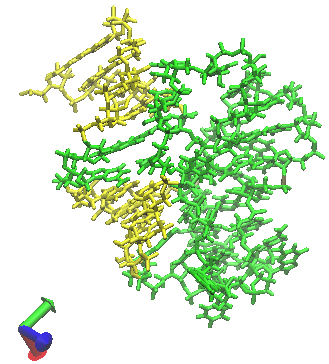
\includegraphics[scale=0.8]{./pictures/motifs_vmd.png}
\caption{Result of running the exemplary structure \texttt{vmd\_run.tcl} script in the VMD program after changing display into \texttt{Orthographic} and changing the background color. }
\end{figure}

\paragraph{Representing hydrogen bonding and stacking on the tertiary structure} The program produces several .pdb files with occupancy column replaced with the values of:
\begin{itemize}
\item \texttt{\_2D.pdb} -- the number of hydrogen bonds in the Watson-Crick pairs created by the given nucleotide.
\item \texttt{\_3D.pdb} -- the number of hydrogen bonds in the non Watson-Crick pairs created by the given nucleotide.
\item \texttt{\_coulomb.pdb} -- the value of the Coulomb energy for a given nucleotide  (the sum of all interactions the nucleotide is involved in).
\item \texttt{\_VDW.pdb} -- the value of the Van der Waals energy for a given nucleotide (the sum of all interactions the nucleotide is involved in).
\item \texttt{\_stacking\_sum.pdb} -- the sum of Van der Waals and Coulomb energies. 
\end{itemize}

In the case of trajectory these .pdb files contain the average values for the analyzed trajectory. \texttt{VMD} is a powerful tool that has a complete user guide and tutorial that can be found on the VMDs home website (\url{http://www.ks.uiuc.edu/Research/vmd/}). Here, we describe a short manual on how to visualize the computed data.

The user has to open the \texttt{VMD} program and load one of the .pdb files, through choosing the \texttt{New Molecule} from the \texttt{File} drop-down menu. As it is shown below:

\begin{figure}[h!]
\centering
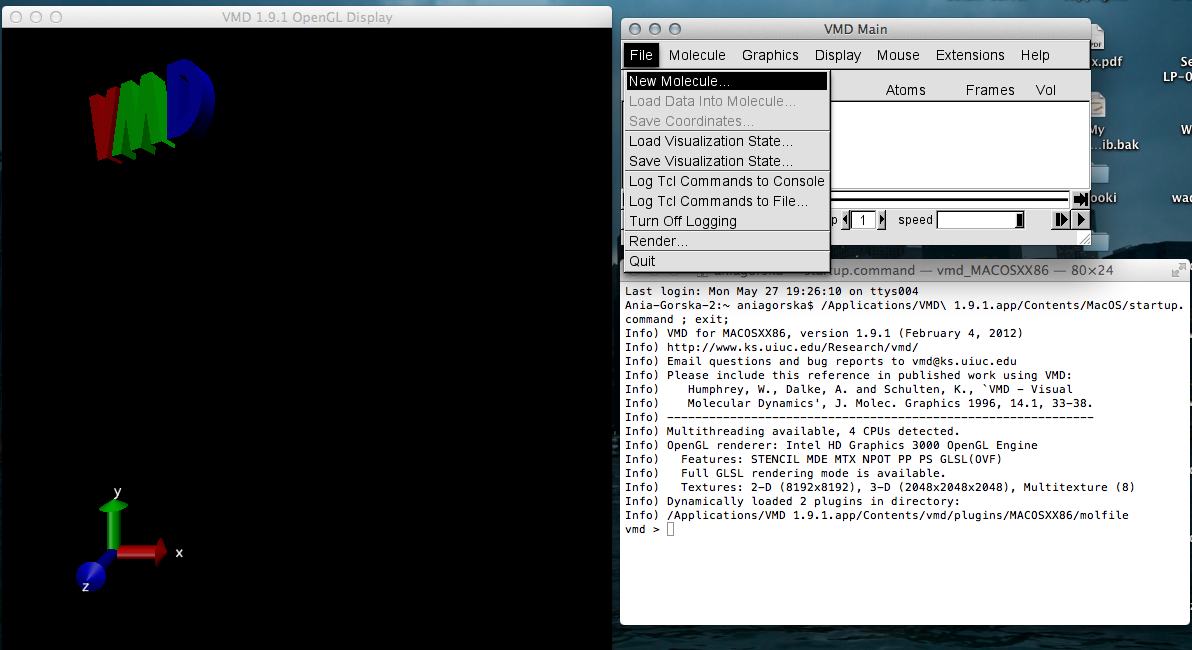
\includegraphics[scale=0.4]{./pictures/vmd1.png}
\end{figure}

Next, one has to \texttt{Browse} and \texttt{Load} a desired .pdb file:
\begin{figure}[h!]
\centering
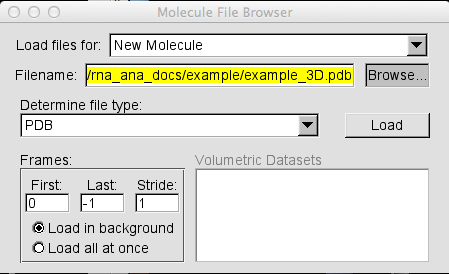
\includegraphics[scale=0.4]{./pictures/vmd2.png}
\end{figure}
\newpage
Having the loaded structure, one needs to open the \texttt{Representations} window from the \texttt{Graphics} drop-down menu:
\begin{figure}[h!]
\centering
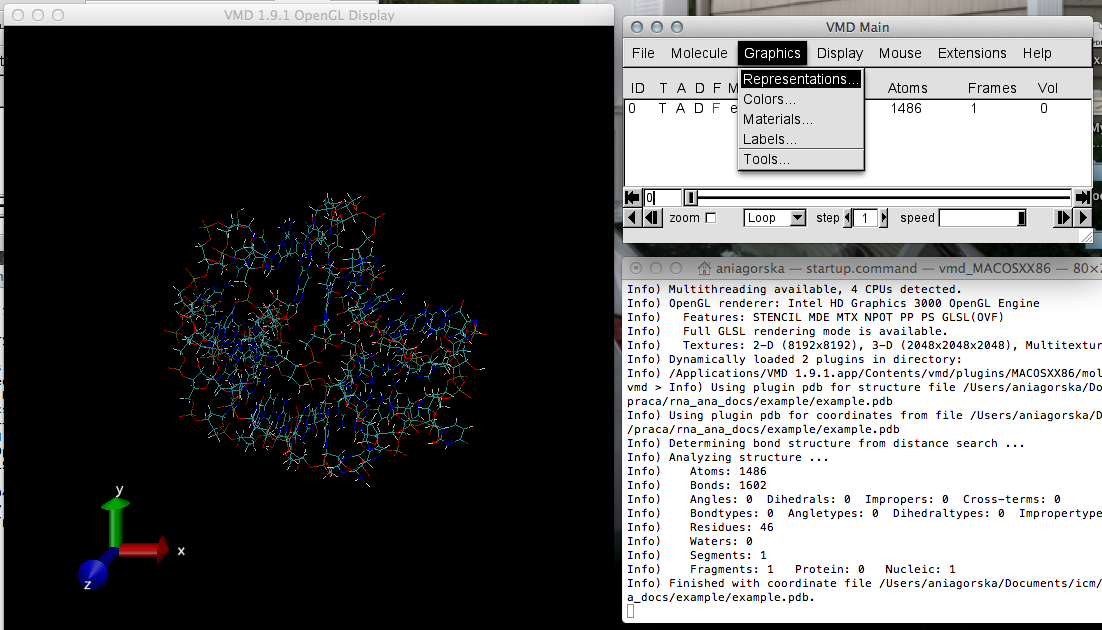
\includegraphics[scale=0.4]{./pictures/vmd3.png}
\end{figure}

The \texttt{Representations} menu allows one to create multiple different representations. To color the structure by the occupancy column from the .pdb file, we propose to change the \texttt{Drawing Methods} into the \texttt{New Cartoon} and the \texttt{Coloring Method} into the \texttt{Occupancy}:

\begin{figure} [h!]
\begin{center}
\subfigure[]{
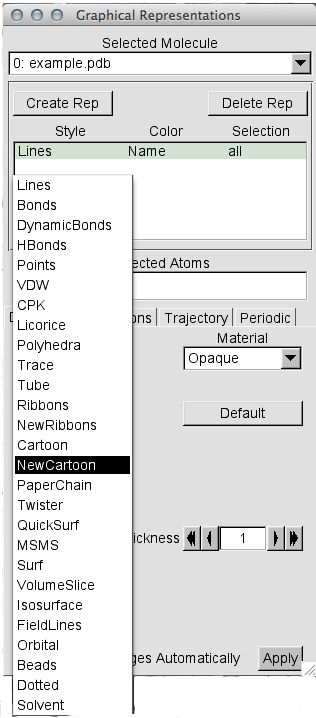
\includegraphics[scale=0.325]{pictures/vmd4.png}}
\subfigure[]{
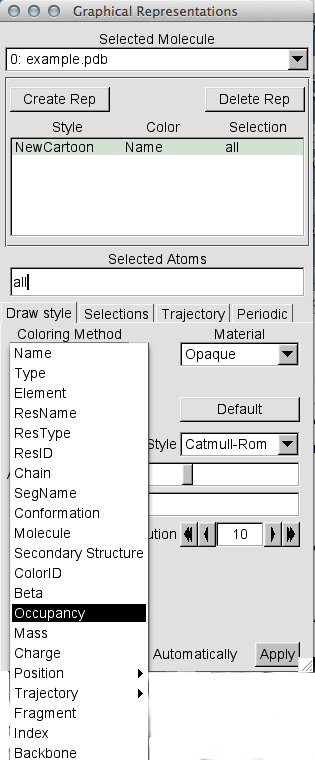
\includegraphics[scale=0.3]{pictures/vmd5.png}}
\end{center}
\end{figure} 
\newpage
Then the color scale can be altered through \texttt{Graphics} $>$ \texttt{Color} $>$ \texttt{Color Scale}:

\begin{figure}[h!]
\centering
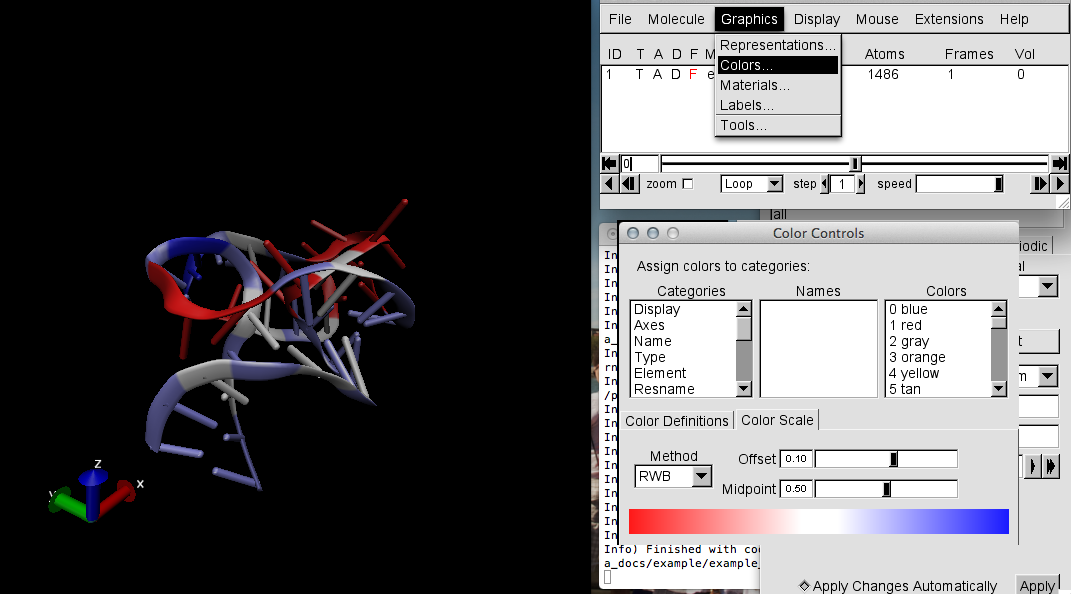
\includegraphics[scale=0.4]{./pictures/vmd6.png}
\end{figure}

If you proceed int the same way with more than one .pdb structure you can use the \texttt{Move} tool (\texttt{Mouse} $>$ \texttt{Move} $>$ \texttt{Molecule}) and view the colored structures at the same time as it is presented in Figure \ref{3Ddifferent}.

\begin{figure}[h!]
\centering
\label{3Ddifferent}
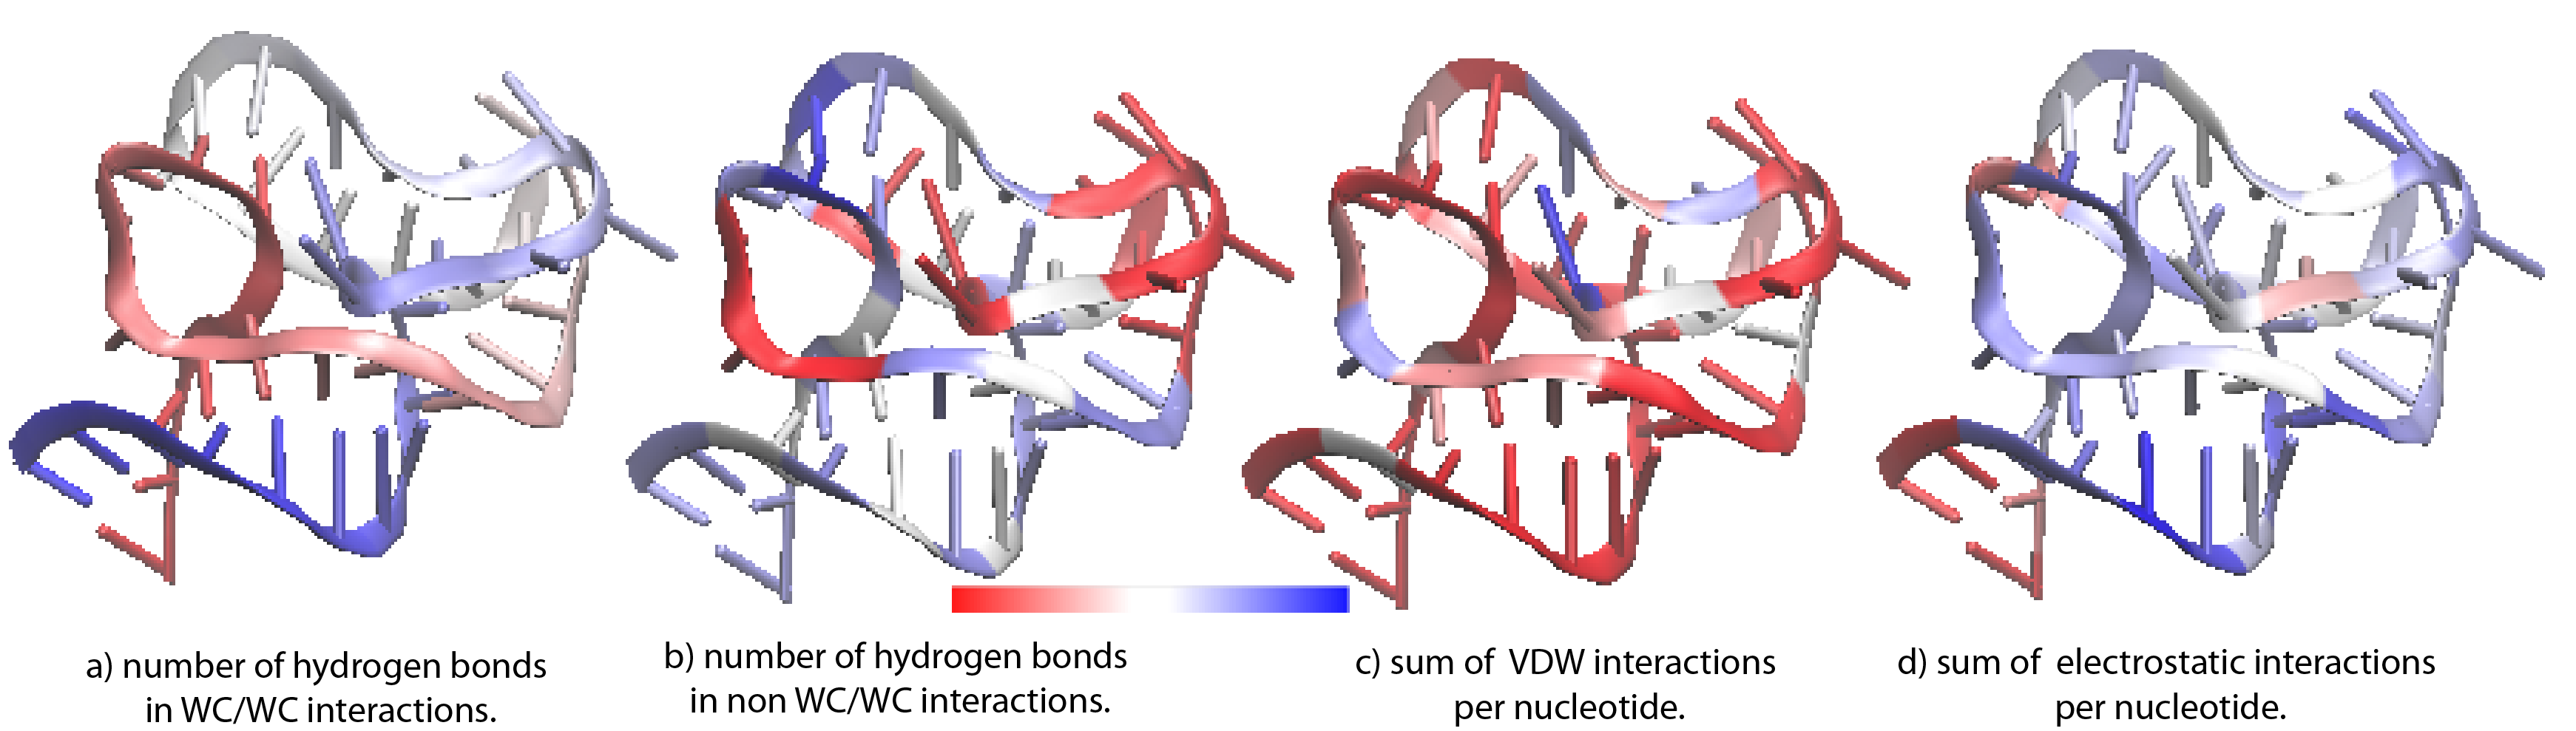
\includegraphics[scale=0.65]{./pictures/3D_different.png}
\end{figure}

\paragraph{Secondary structure trajectory} can be visualized with the RNAMovies \cite{Evers1999} program. The MINT returns the \texttt{RNAStructML.xml} containing the trajectory of the secondary structure. For every frame the dot-bracket representation is written into the .xml file. This allows to produce the movie of the secondary structure trajectory. 

The RNAMovies \cite{Evers1999}  java .jar file can be downloaded from its home page: \url{http://bibiserv.techfak.uni-bielefeld.de/rnamovies/}. Here we present a short tutorial on how to open a .xml file and view the trajectory.

First, one has to open the RNAMovies and choose the \texttt{Import} option from the \texttt{File} drop-down menu. 
\begin{figure}[h!]
\centering
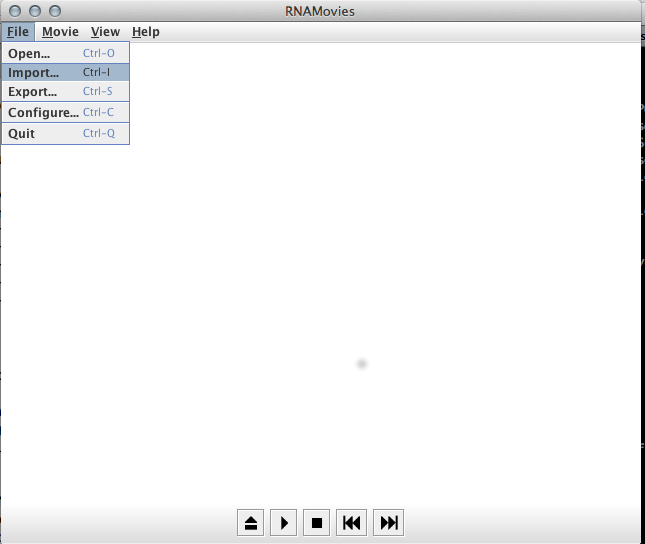
\includegraphics[scale=0.4]{./pictures/RNAmovies_1.png}
\end{figure}
\newpage
Find a proper .xml file in your disk, and click \texttt{Open}:
\begin{figure}[h!]
\centering
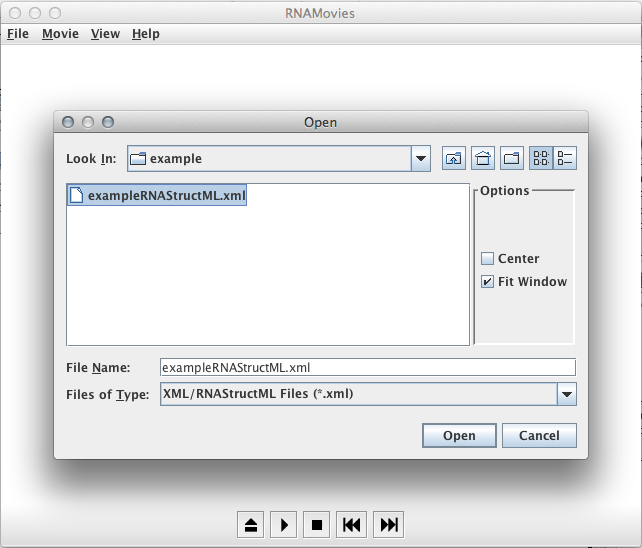
\includegraphics[scale=0.4]{./pictures/RNAmovies_2.png}
\end{figure}

One can navigate the trajectory using the arrows in the bottom of the window. If you want to loop the trajectory or change the pace go to the \texttt{File} $>$ \texttt{Configure} menu: 
\begin{figure}[h!]
\centering
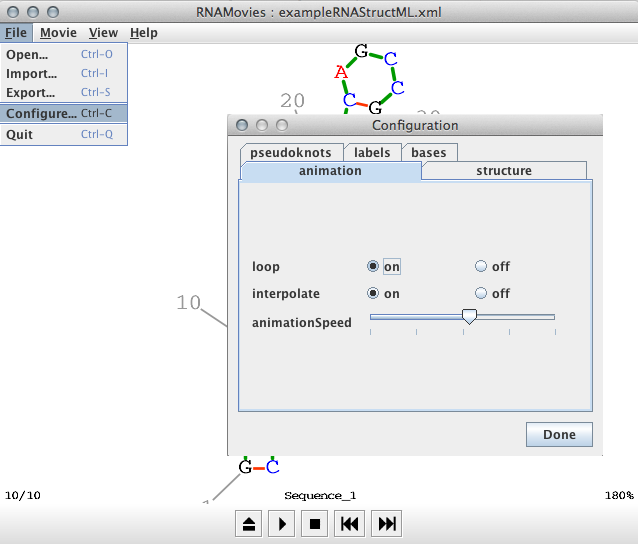
\includegraphics[scale=0.4]{./pictures/RNAmovies_3.png}
\end{figure}
\newpage
The animated trajectory can be written into the .gif file  (\texttt{File} $>$ \texttt{Export}).

\subsection{Correlations}
In the \texttt{MINT} directory user can find additional python script \texttt{CORRELATIONS.py} computing \texttt{phi coefficient} for every pair of nucleotides in the structure. The \texttt{phi coefficient} is computed using the equation:
\begin{center}
\begin{large}
$ \phi = \frac{n_{11}n_{00}}{\sqrt{n_{\bullet1}n_{\bullet0} n_{0\bullet}n_{1\bullet}}}$
\end{large}
\end{center}

where:
\begin{itemize}
\item $n_{11}$ is a number of frames when both nucleotides are creating WCWC pair.
\item $n_{00}$ is a number of frames when none of the nucleotides is creating WCWC pair.
\item $n_{01}$ is a number of frames when first of the nucleotides is creating WCWC pair and the second nucleotide is not, analogously $n_{10}$ is the number of frames when first nucleotide is paired and second is free.
\end{itemize}

and:
\begin{itemize}
\item $n_{\bullet1} = n_{11}+n_{01}$
\item $n_{1\bullet} = n_{11}+n_{10}$
\item $n_{\bullet0} = n_{00}+n_{10}$
\item $n_{0\bullet} = n_{00}+n_{01}$
\end{itemize}

\begin{figure}[h!]
\label{coefficient}
\centering
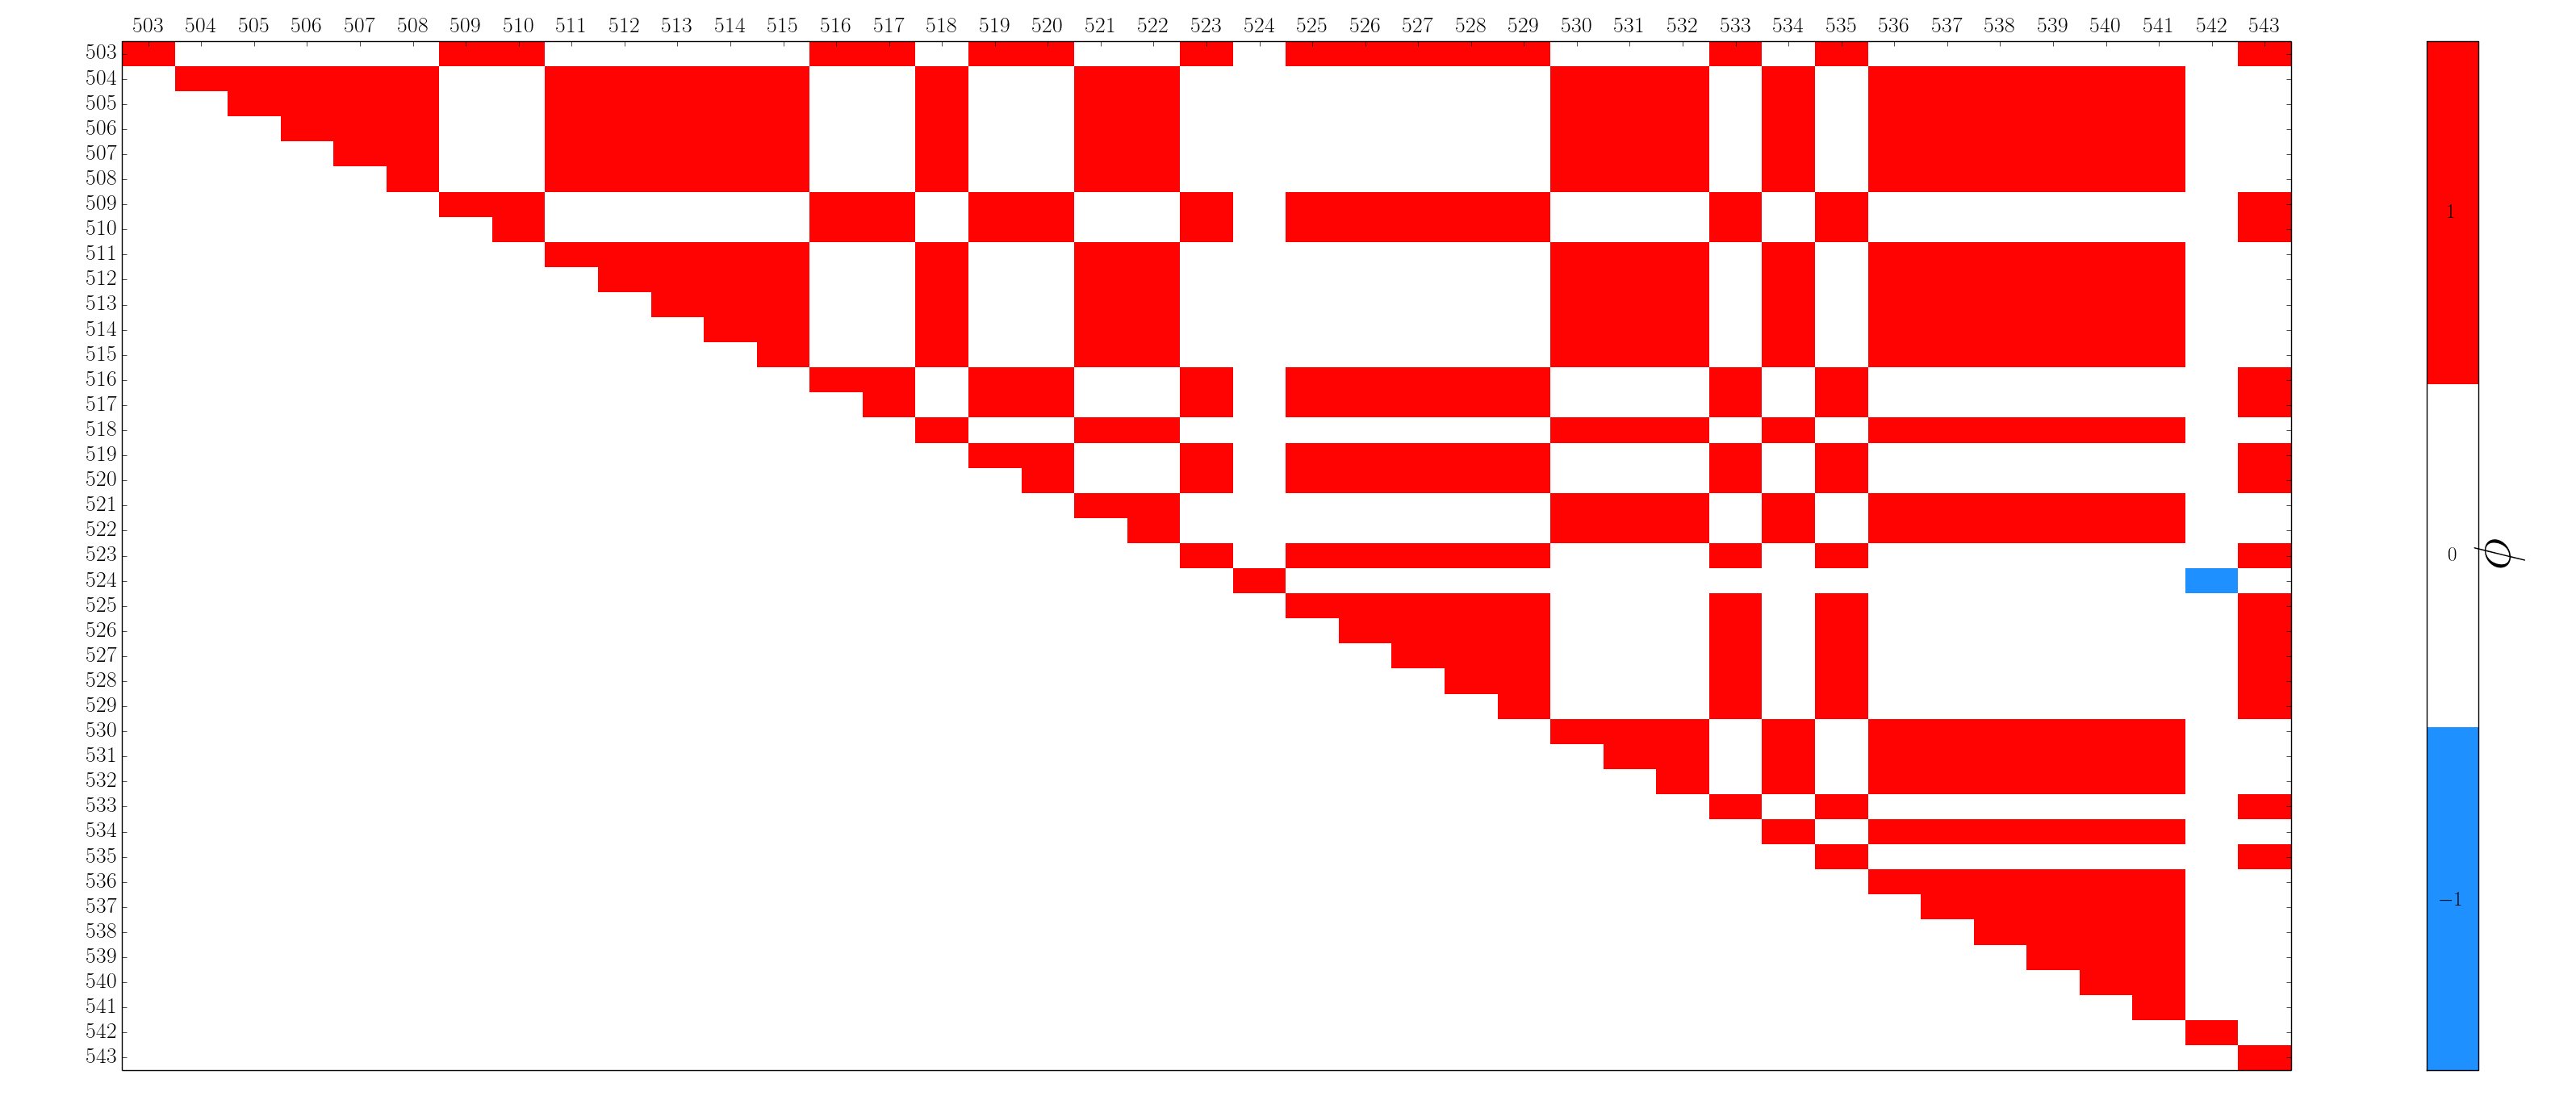
\includegraphics[scale=0.4]{./pictures/correlation_matrix.png}
\caption{Heap map of \texttt{phi coefficient} for the the same exemplary molecule as shown before, and for discussed trajectory. These map was calculated with 0.4 \texttt{cutoff}.}
\end{figure}

\texttt{Phi coefficient} takes values between -1 and 1. It is believed that when coefficient value is close to 0 the correlation is not reliable. In the heat map, all values larger then \texttt{cutoff} will be marked red, all lower than \texttt{-1*cutoff} are marked blue. The rest will remain white. The level of \texttt{cutoff} is defined by the user.

The script produces a matrix that is both written into the text file and printed in the form of the heat map. Figure \ref{coefficient} presents heat map of \texttt{phi coefficient} for the previously discussed exemplary RNA molecule and its 10 frame molecular dynamics.

\texttt{CORRELATIONS.py} script uses as an input the \texttt{MINT} output: \texttt{pairs\_in\_time.csv} type, cutoff and list of numbers of nucleotides you want to compute the coefficient for:\\

\texttt{ python pairs\_correlations.py step6\_pairs\_in\_time.csv 0.4 "[(1210,1220),(985,995), (1043,1047)]"} \\

The list of nucleotides has to be specified in the square brackets and quotation marks. Inside round brackets the ranges of nucleotides must be specified. 

If the user wants to compute the phi coefficient for all nucleotides should not specify list of nucleotides like:\\
\texttt{ python pairs\_correlations.py step6\_pairs\_in\_time.csv 0.4 } \\

Heat map is only printed for the half of the matix, another half would be identical. All of the nucleotides are correlated with themselves - the diagonal is colored red. All of the nucleotides creating WCWC pairs with each other are also positively correlated. The neighboring pairs that work together will also be visible as correlated in all to all manner. The negative correlation suggests that there are pairs that opens when another one closes.


\section{Appendices}
\begin{appendices}
\subsection{Adding hydrogens to a .pdb structure}

Following the Leontis and Westhof \cite{Leontis2002} classification of interacting nucleotides, our program searches for hydrogen bonds in the given structure. In order to properly recognize all the hydrogen bonds, the hydrogen atoms have to be present in the input .pdb file. If one analyzes the files from MD simulations, the hydrogen atoms were added to the structure during the preparation of an MD run, according to the atom type definitions in the force field. Various tools of the MD packages can be used to assign the positions of hydrogens (for example Xleap from AmberTools). 

However, if a structure from the PDB database has to be analyzed and the user does not have experience with MD methods, hydrogen atoms can be added using on-line servers. We have tested a few of them and we can recommend the Molprobility service~\cite{Chen2010} (\url{http://molprobity.biochem.duke.edu/}). It works even with the structures as large as the ribosomal subunits in an acceptable time span. What is more, the software can be downloaded from the \url{http://kinemage.biochem.duke.edu/software/reduce.php} website and used offline.

\end{appendices}
\bibliography{bibliografia}
\bibliographystyle{plain}
\end{document}